\begin{figure}
			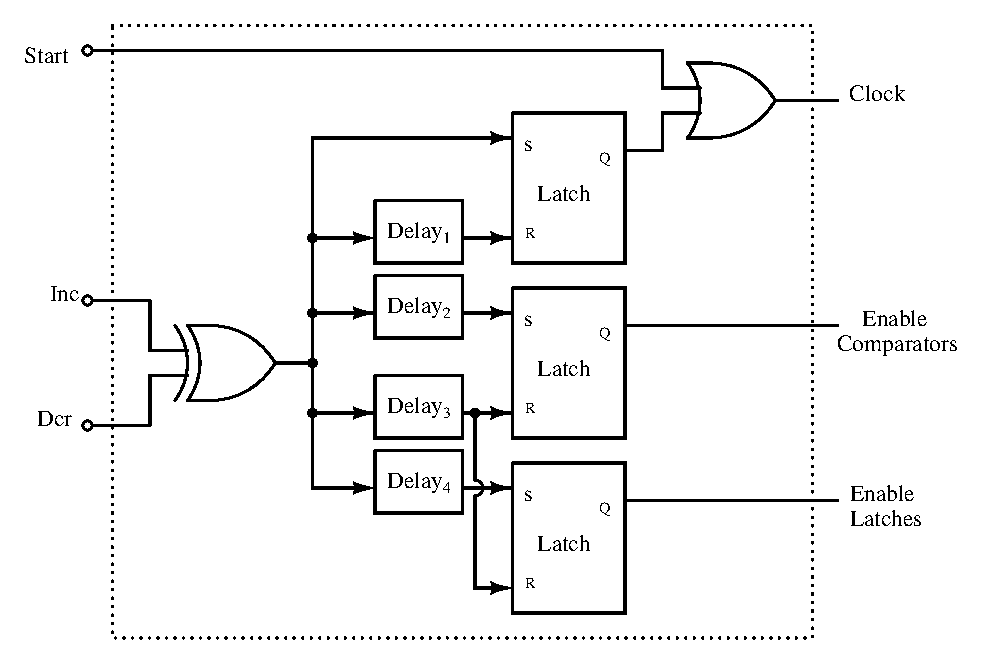
\includegraphics[width=5cm,height=5cm,angle=360]{Figures/FlashControllerCircuit.ps}\\
		\end{figure}
		\small{Block Diagram of Controller Circuit}



		\begin{columns}[c]
		\column{2.5in}
			\begin{figure}
				\begin{center}
					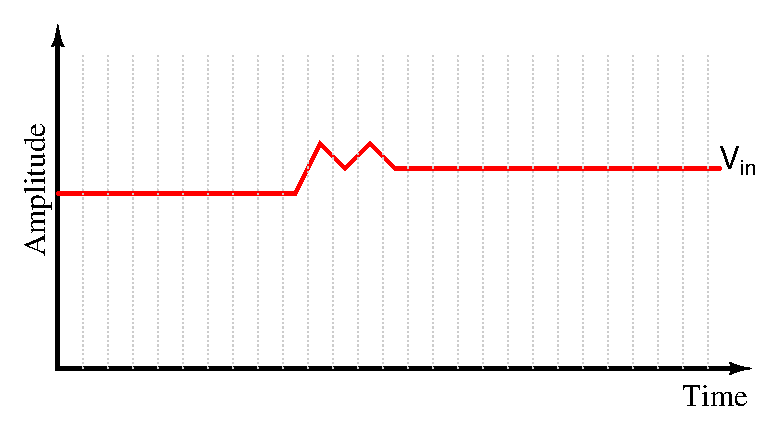
\includegraphics[width=6cm,height=4cm,angle=360]{Figures/BriefVariation.ps}\\
               				\caption{Some Signals almost always constant and may vary only during brief moments.}
				\end{center}
			\end{figure}
		\column{2.5in}
			\begin{figure}
				\begin{center}
					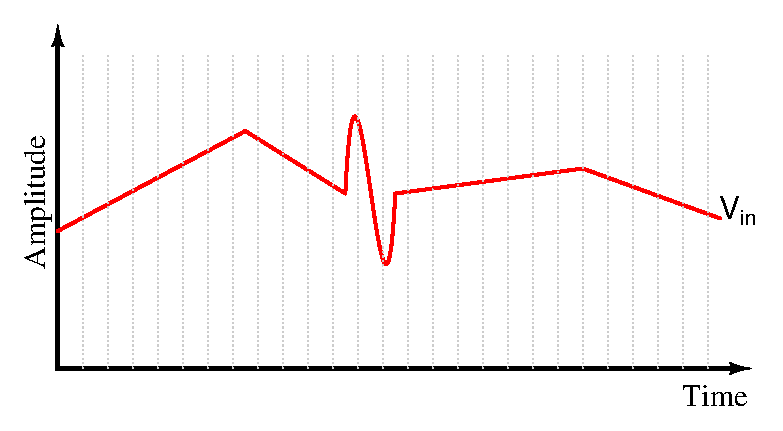
\includegraphics[width=6cm,height=4cm,angle=360]{Figures/HighFrequncy.ps}\\
               				\caption{Some Signals Maximum frequency very high compared to the normal frequency.}
				\end{center}
			\end{figure}
		\end{columns}







\section{Motivation}
\subsection*{Motivation}
\begin{frame}
	\frametitle{Introduction}
	\begin{center}
		Signals have interesting statistical properties	
	\end{center}
	\begin{center}
		\begin{columns}[c]
		\column{2.5in}
			\begin{figure}
				\begin{center}
					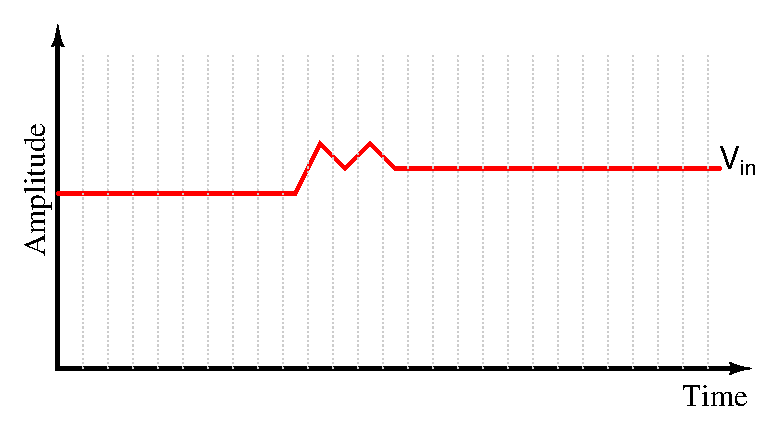
\includegraphics[width=6cm,height=4cm,angle=360]{Figures/BriefVariation.ps}\\
               				\caption{Some Signals almost always constant and may vary only during brief moments.}
				\end{center}
			\end{figure}
		\column{2.5in}
			\begin{figure}
				\begin{center}
					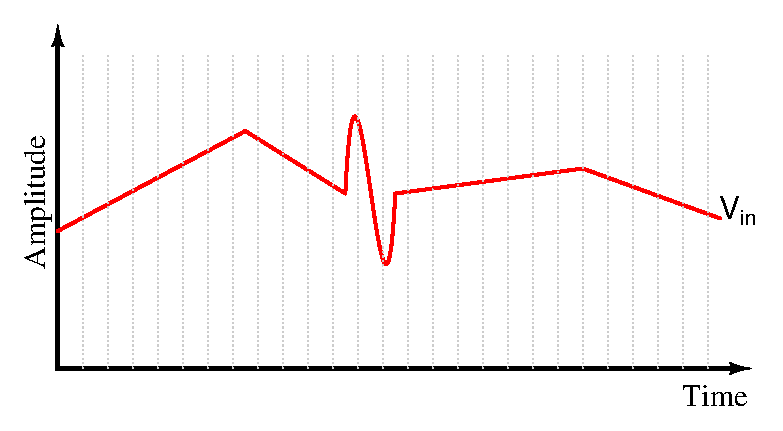
\includegraphics[width=6cm,height=4cm,angle=360]{Figures/HighFrequncy.ps}\\
               				\caption{Some Signals Maximum frequency very high compared to the normal frequency.}
				\end{center}
			\end{figure}
		\end{columns}
	\end{center}
\end{frame}










		\begin{itemize}
		\item{Signals have interesting statistical properties.}\\
		\item{Some Signals almost always constant and may vary significantly only during brief moments.}\\
		\item{Some Signals Maximum frequency very high compared to the normal frequency.}
 		\end{itemize}


\begin{columns}[c]
			\column{3.0in}
			\begin{itemize}
				\item{Motivation for VTQ ADC is TIQ ADC}
       				\item{Power can be reduced by reducing no. of comparators}
       				\item{This also eliminates decoding logic}
 			\end{itemize}
			\column{2.0in}
			\begin{figure}
				\begin{center}
					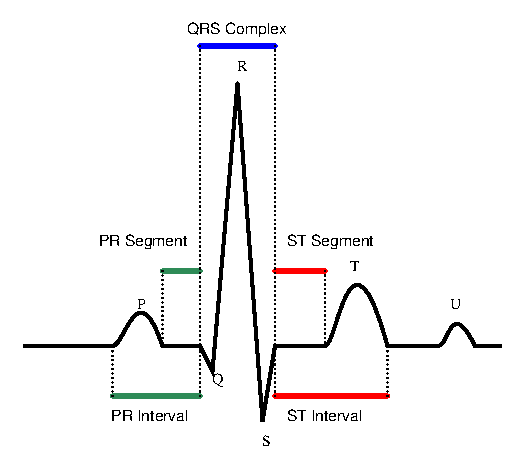
\includegraphics[width=5cm,height=5cm,angle=360]{Figures/ElectroCardioGraphy.ps}\\
               				\small{Block Diagram of TIQ ADC}
				\end{center}
			\end{figure}
		\end{columns}











\section{Variable Threshold Quantization ADC}
\subsection*{Motivation}
\begin{frame}
	\frametitle{Motivation for VTQ ADC}
	\begin{center}
		\begin{columns}[c]
		\column{2.5in}
			\begin{itemize}
				\small{\item{Motivation for VTQ ADC is TIQ ADC}
       				\item{Power can be reduced by reducing no. of comparators}
       				\item{This also eliminates decoding logic}}
 			\end{itemize}
				\begin{figure}
					\begin{center}
				\includegraphics[width=4.5cm,height=2.5cm,angle=360]{EPSFiles/TIQ_COM.eps}\\
                		%\caption{TIQ Comparator}
					\end{center}
				\end{figure}
			\begin{center}
			\small{TIQ Comparator Circuit}
			\end{center}
		\column{2.5in}
			\begin{figure}
				\begin{center}
				\includegraphics[width=5cm,height=5cm,angle=360]{EPSFiles/TIQ_ADC.eps}\\
               			\small{Block Diagram of TIQ ADC}
				\end{center}
			\end{figure}
		\end{columns}
	\end{center}	
\end{frame}
%-----------------------------------------------%
%-----------------------------------------------%
\subsection*{Block Diagram of Proposed VTQ ADC}
\begin{frame}
	\frametitle{Block Diagram of Proposed VTQ ADC}
	\begin{center}
		\begin{figure}
		\includegraphics[width=9cm,height=5cm,angle=360]{EPSFiles/VTQ_ADC.eps}\\
		\end{figure}
	\small{Block Diagram of the Proposed VTQ Architecture for 6-bit ADC}
	\end{center}
\end{frame}
%-----------------------------------------------%
%-----------------------------------------------%
\begin{frame}
	\frametitle{Circuit Diagram of VTQ Comparator (MSB-2)}
	\begin{center}
		\begin{figure}
		\includegraphics[width=9cm,height=5cm,angle=360]{EPSImages/VTQ_COMA.eps}\\
		\end{figure}
	\small{Circuit Diagram of VTQ Comparator (MSB-2)}
	\end{center}
\end{frame}
%-----------------------------------------------%
%-----------------------------------------------%
\begin{frame}
	\frametitle{Construction of VTQ Comparator (MSB-2)}
	\begin{center}
		\begin{figure}
		\includegraphics[width=9cm,height=5cm,angle=360]{EPSImages/VTQ_COMB.eps}\\
		\end{figure}
	\small{Construction of VTQ Comparator (MSB-2)}
	\end{center}
\end{frame}
%-----------------------------------------------%
%-----------------------------------------------%
\subsection*{Simulation Results of Proposed VTQ ADC}
\begin{frame}
	\frametitle{Simulation Results of Proposed VTQ ADC}
	\begin{center}
		\begin{figure}
		\includegraphics[width=9cm,height=6cm,angle=360]{EPSImages/VTQ_SIM1.eps}\\
		\end{figure}
	\end{center}
\end{frame}
%-----------------------------------------------%
%-----------------------------------------------%
\subsection*{Extentions to Proposed VTQ Comparator}
\begin{frame}
	\frametitle{Block Diagram of VTQ Based SAR ADC}
	\begin{center}
		\begin{figure}
		\includegraphics[width=9cm,height=5cm,angle=360]{EPSFiles/VTQ_SAR.eps}\\
		\end{figure}
	\small{Block Diagram of VTQ Based SAR ADC Architecture for 6-bit}
	\end{center}
\end{frame}
%-----------------------------------------------%
%-----------------------------------------------%
\begin{frame}
	\frametitle{Block Diagram of VTQ Based DAC}
	\begin{center}
		\begin{figure}
		\includegraphics[width=9cm,height=5cm,angle=360]{EPSImages/VTQ_DAC.eps}\\
		\end{figure}
	\small{Circuit Diagram of VTQ Based DAC Architecture for  2-bit}
	\end{center}
\end{frame}
%-----------------------------------------------%
%-----------------------------------------------%
%---------------------------------------------------------------------------------------------------------------%
\section{TIQ Based Succsive Aproximation ADC}
\subsection*{Motivation}
\begin{frame}
	\frametitle{Motivation for TIQ Based SAR ADC}
	\begin{center}
		\begin{columns}[c]
		\column{3.25in}
			\begin{itemize}
				\small{\item{Motivation for TIQ Based SAR ADC is TIQ Comparator}
       				\item{Power can be reduced by reducing no. of active comparators}}
 			\end{itemize}
			\begin{figure}
				\begin{center}
				\includegraphics[width=7cm,height=3cm,angle=360]{EPSFiles/TIQ_VTC.eps}\\
				\small{TIQ Comparator VT Charecteristics}
                		\end{center}
			\end{figure}			
		\column{1.75in}
			\begin{figure}
				\begin{center}
				\includegraphics[width=3.5cm,height=3.5cm,angle=360]{EPSFiles/TIQ_COM.eps}\\
               			\small{TIQ Comparator}
				\end{center}
			\end{figure}
		\end{columns}
	\end{center}	
\end{frame}
%-----------------------------------------------%
%-----------------------------------------------%
\subsection*{Block Diagram of TIQ Based SAR ADC }
\begin{frame}
	\frametitle{Block Diagram of TIQ Based SAR ADC}
	\begin{center}
		\begin{figure}
		\includegraphics[width=9cm,height=5cm,angle=360]{EPSFiles/SAR_ADC.eps}\\
		\end{figure}
	\small{Block Diagram of TIQ Based Succsive Aproximation ADC}
	\end{center}
\end{frame}
%-----------------------------------------------%
%-----------------------------------------------%
\begin{frame}
	\frametitle{Components of TIQ Based SAR ADC}
	\begin{center}
		\begin{figure}
		\includegraphics[width=8cm,height=5cm,angle=360]{EPSImages/SAR_COMA.eps}\\
		\end{figure}
	\small{Circuit Diagram of Comparators used in Comparator Array}
	\end{center}
\end{frame}
%-----------------------------------------------%
%-----------------------------------------------%
\begin{frame}
	\frametitle{Components of TIQ Based SAR Controller}
	\begin{center}
		\begin{figure}
		\includegraphics[width=10cm,height=6cm,angle=360]{EPSImages/SAR_CON.eps}\\
		\end{figure}
	\end{center}
\end{frame}
%-----------------------------------------------%
%-----------------------------------------------%
\subsection*{Simulation Results of SAR Controler}
\begin{frame}
	\frametitle{Simulation Results of SAR Controler}
	\begin{center}
		\begin{figure}
		\includegraphics[width=9cm,height=6cm,angle=360]{EPSImages/SAR_SIM1.eps}\\
		\end{figure}
	\end{center}
\end{frame}
%-----------------------------------------------%
%-----------------------------------------------%
\begin{frame}
	\frametitle{Simulation Results of SAR Controler}
	\begin{center}
		\begin{figure}
		\includegraphics[width=9cm,height=6cm,angle=360]{EPSImages/SAR_SIM2.eps}\\
		\end{figure}
	\end{center}
\end{frame}
%-----------------------------------------------%
%-----------------------------------------------%
%---------------------------------------------------------------------------------------------------------------%
\section{Extending Analog Input Range of TIQ ADC }
\subsection*{Motivation}
\begin{frame}
	\frametitle{Motivation for EAIR for TIQ ADC}
	\begin{center}
		\begin{columns}[c]
		\column{2.5in}
			\begin{itemize}
				\small{\item{Motivation for EAIR for TIQ ADC is VTQ Comparator}
				\item{$Maximum\ Analog\ range=V_{dd}-(V_{tn}+|V_{tp}|)$}
				\item{Large widths of transistors are required to get $V_{ref}$}
       				}
 			\end{itemize}
			\begin{figure}
				\begin{center}
				%\includegraphics[width=5cm,height=3cm,angle=360]{EPSFiles/TIQ_COM.eps}\\
				%\small{TIQ Comparator}
                		\end{center}
			\end{figure}			
		\column{2.5in}
			\begin{figure}
				\begin{center}
				\includegraphics[width=5cm,height=5cm,angle=360]{EPSFiles/TIQ_ADC.eps}\\
               			\small{TIQ Comparator}
				\end{center}
			\end{figure}
		\end{columns}
	\end{center}	
\end{frame}
%-----------------------------------------------%
%-----------------------------------------------%
\begin{frame}
	\frametitle{Motivation for EAIR for TIQ ADC}
	\begin{center}
		\begin{figure}
		\includegraphics[width=10cm,height=5cm,angle=360]{EPSImages/VAR_VTH.eps}\\
		\small{Variation of Vref with Width of Mosfets}
		\end{figure}	
	\end{center}
\end{frame}
%-----------------------------------------------%
%-----------------------------------------------%
\subsection*{Block Diagram of Proposed ADC}
\begin{frame}
	\frametitle{Block Diagram of Proposed ADC for EAIR for TIQ ADC}
	\begin{center}
		\begin{figure}
		\includegraphics[width=5cm,height=5cm,angle=360]{EPSFiles/PRO_ADC.eps}\\
		\small{Block Diagram of Proposed ADC for EAIR TIQ ADC}
		\end{figure}	
	\end{center}
\end{frame}
%-----------------------------------------------%
%-----------------------------------------------%
\begin{frame}
	\frametitle{Block Diagram of Proposed ADC for EAIR for TIQ ADC}
	\begin{center}
		\begin{columns}[c]
		\column{2.5in}
			\begin{figure}
			\includegraphics[width=4cm,height=4cm,angle=360]{EPSFiles/PRO_COP.eps}\\
			\small{Comparator to increase $V_{ref}$}
			\end{figure}	
		\column{2.5in}
			\begin{figure}
			\includegraphics[width=4cm,height=4cm,angle=360]{EPSFiles/PRO_CON.eps}\\
			\small{Comparator to decrease $V_{ref}$}
			\end{figure}
		\end{columns}
	\end{center}
\end{frame}
%-----------------------------------------------%
%-----------------------------------------------%
\begin{frame}
	\frametitle{Block Diagram of Proposed ADC for EAIR for TIQ ADC}
	\begin{center}
		\begin{figure}
		\includegraphics[width=8cm,height=6cm,angle=360]{EPSImages/EAR_ADC.eps}\\
		\end{figure}	
	\end{center}
\end{frame}
%-----------------------------------------------%
%-----------------------------------------------%

%---------------------------------------------------------------------------------------------------------------------------%

%\begin{frame}
%	\frametitle{Proposed Architecture to Reduce Data}  \footnotesize
%	\begin{center}
%		\begin{figure}
%			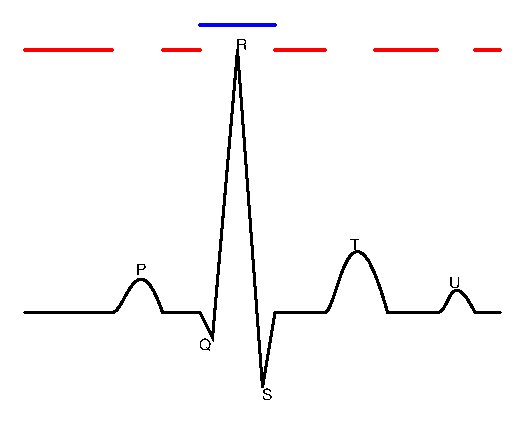
\includegraphics[width=7 cm,height=5 cm,angle=360]{Figures/09ECGSignal.ps}\\
%		\end{figure}
%		\scriptsize{ \color{blue}{Block Diagram of the Proposed ADC Architecture to reduce Data}}
%	\end{center}
%\end{frame}
%---------------------------------------------------------------------------------------------------------------------------%
%\begin{frame}
%	\frametitle{Drawbacks of Level Cross Sampling ADC} \footnotesize
%	\begin{center}
%		\begin{itemize}
%			\item{Requires Separate Clock Generation Circuit for Timer} \\
%				\begin{itemize}
%					\scriptsize{ \color{red}\item{Increases in Design Complexity}} \\
%					\scriptsize{ \color{blue}\item{Architecture Should work with Synchronous Clock}} \\
%				\end{itemize}
%			\item{It Follows Successive Approximation to Track the input Signal} \\
%				\begin{itemize}
%					\scriptsize{ \color{red}\item{Unable to Follow input Signal}} \\
%					\scriptsize{ \color{blue}\item{Increase the speed of Tracking with more no. of Bits}} \\
%				\end{itemize}	
%			\item{Once Designed for particular signal can't be used for other signals} \\
%				\begin{itemize}
%					\scriptsize{ \color{red}\item{Reduction in Power Efficiency}} \\
%					\scriptsize{ \color{blue}\item{Use of Variable Resolution Architecture}} \\
%				\end{itemize}
%			\item{Most of the CAD tools don't Support Asynchronous Design} \\
%				\begin{itemize}
%					\scriptsize{ \color{red}\item{Increases in Design Complexity}} \\
%					\scriptsize{ \color{blue}\item{Architecture Should work with Synchronous Clock}} \\
%				\end{itemize}
%		\end{itemize}
%	\end{center}
%\end{frame}


%---------------------------------------------------------------------------------------------------------------------------%
\begin{frame}
	\frametitle{Variable Resolution A to D Converter}  \footnotesize
	\begin{center}
		\begin{figure}
			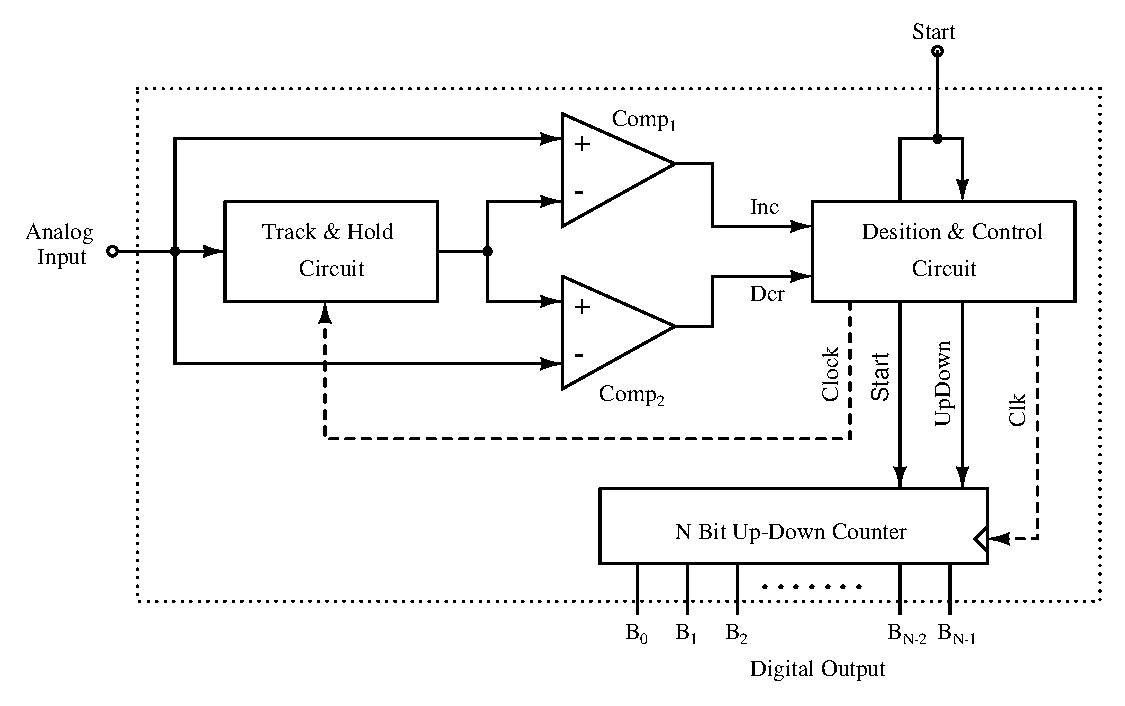
\includegraphics[width=10cm,height=6cm,angle=360]{Figures/AnalogDigitalCounter.ps}\\
		\end{figure}
		\scriptsize{ \color{blue}{Block Diagram of the Variable Resolution ADC Using Up-Down Counter}}
	\end{center}
\end{frame}
%---------------------------------------------------------------------------------------------------------------------------% 
\begin{frame}
	\frametitle{Variable Resolution A to D Converter}  \footnotesize
	\begin{center}
		\begin{figure}
			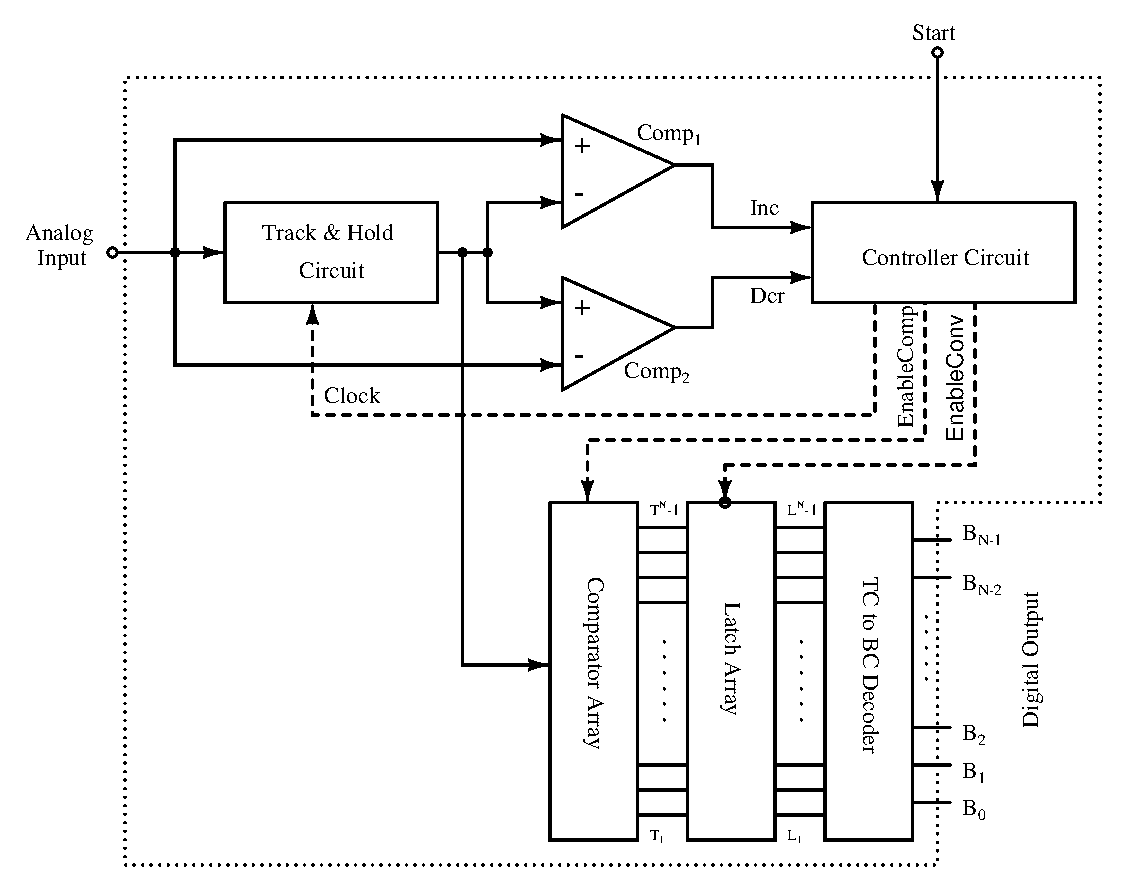
\includegraphics[width=10cm,height=6cm,angle=360]{Figures/FlashAnalogDigitalCounter.ps}\\
		\end{figure}
		\scriptsize{ \color{blue}{Block Diagram of the Variable Resolution ADC Using Flash ADC}}
	\end{center}
\end{frame}



\section{Conclusion and Future Work}
\begin{frame}
	\frametitle{Variable Resolution A to D Converter}  \footnotesize
	\begin{center}
		\begin{figure}
			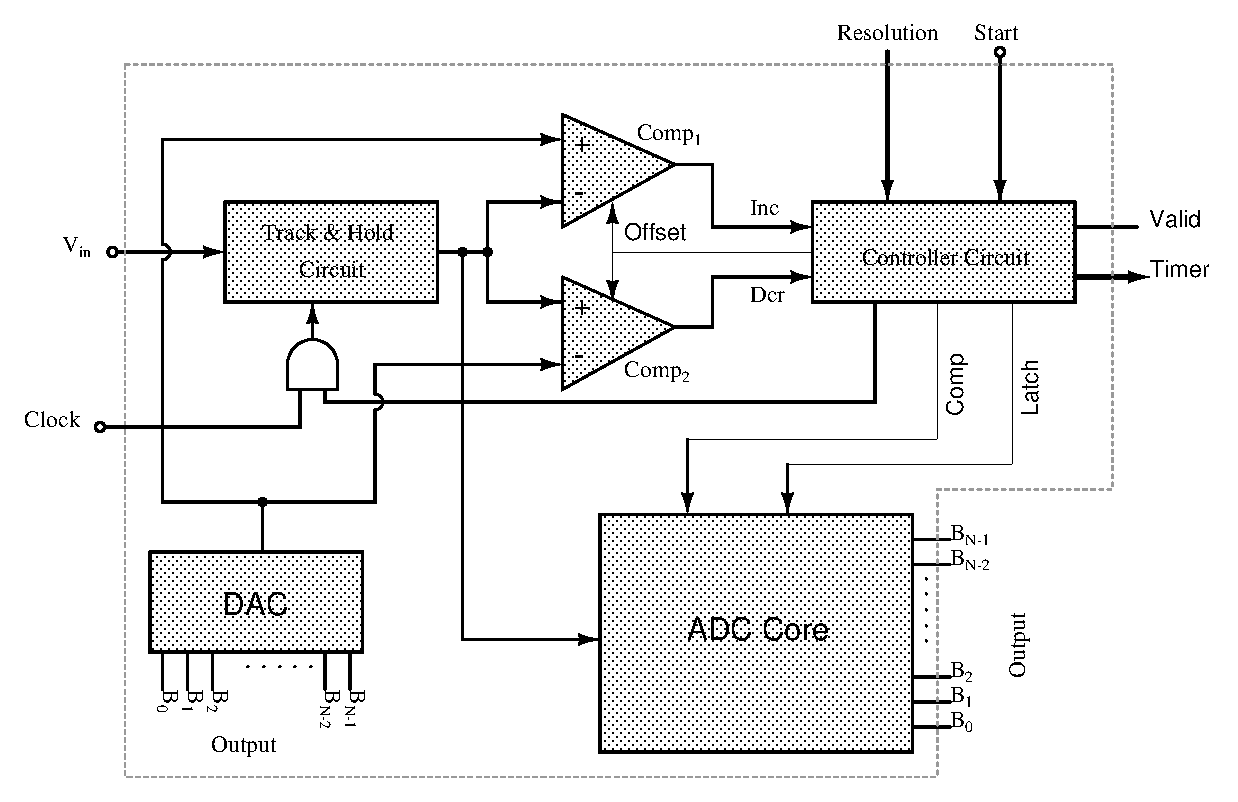
\includegraphics[width=10 cm,height=5 cm,angle=360]{Figures/14VRADCPower.ps}\\
		\end{figure}
		\scriptsize{ \color{blue}{Block Diagram of the Proposed ADC Architecture for Variable Resolution}}
	\end{center}
\end{frame}





%---------------------------------------------------------------------------------------------------------------------------%
\subsection*{Controller for high activity ratio signals}
\begin{frame}
	\frametitle{Level Cross Sampling vs Nyquist Sampling} \scriptsize
	\footnotesize{When Increment Signal Generated from Difference Quantificator}
	\begin{center}
		\begin{itemize} \scriptsize
			\item{SAR is assigned with all MS bits to '1' untill first '0' and remaing bits are set to '0'}
			\item{Shift Register is assigned with with all '0' except the first '0' in SAR bit is set to '1'}
			\item{\color{blue}Example: \color{black}If contents of SAR are 11\color{brown}0\color{black}10110 \\ 
			\hspace {1.2 cm} Value assigned to Shift Register 00\color{red}1\color{black}00000 \\ 
			\hspace {1.2 cm} Value assigned to SAR 11000000} \\
		\end{itemize}
	\end{center}
	\footnotesize{When Decrement Signal Generated from Difference Quantificator}
	\begin{center}
		\begin{itemize} \scriptsize
			\item{SAR is assigned with all bits set to '0'}
			\item{Shift Register is assigned with with all '0' except the first '1' in SAR bit is set to '1'}
			\item{\color{blue}Example: \color{black}If contents of SAR are 000\color{brown}1\color{black}0110 \\ 
			\hspace {1.2 cm} Value assigned to Shift Register 000\color{red}1\color{black}0000 \\ 
			\hspace {1.2 cm} Value assigned to SAR 00000000 }
		\end{itemize}
	\end{center}
\end{frame}
%---------------------------------------------------------------------------------------------------------------------------%


%---------------------------------------------------------------------------------------------------------------------------%
\begin{frame}
	\frametitle{Simulation results} \footnotesize
	\begin{center}
		\begin{figure}
			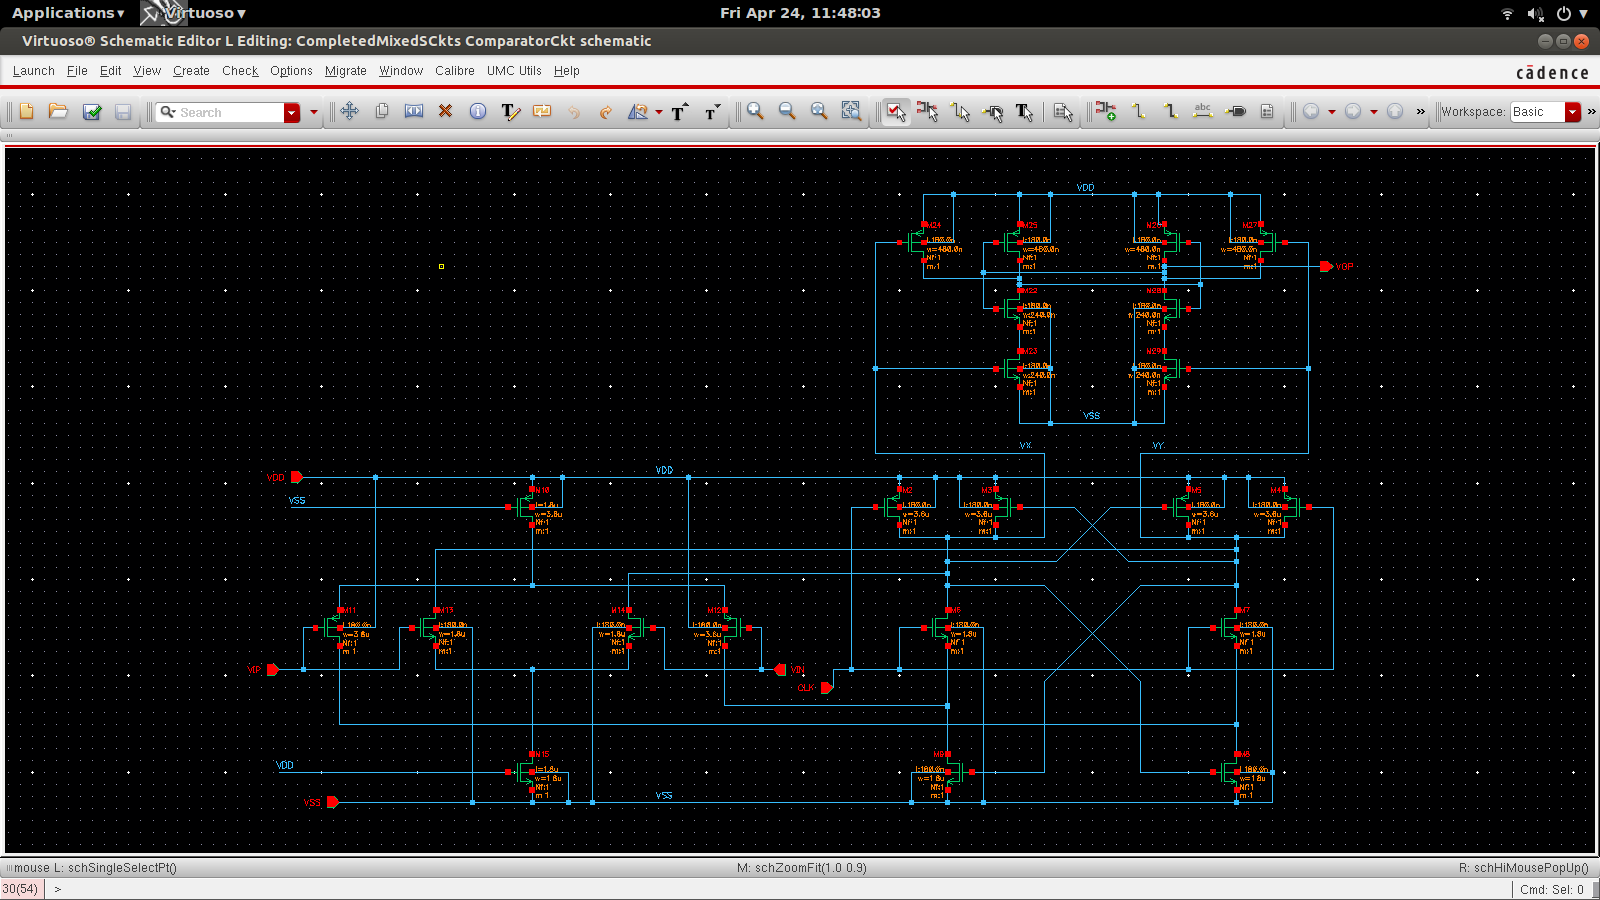
\includegraphics[width=10 cm]{Figures/CCMP.png}\\
		\end{figure}
		\scriptsize{ \color{blue}{}}
	\end{center}
\end{frame}
%---------------------------------------------------------------------------------------------------------------------------%
\begin{frame}
	\frametitle{Simulation results} \footnotesize
	\begin{center}
		\begin{figure}
			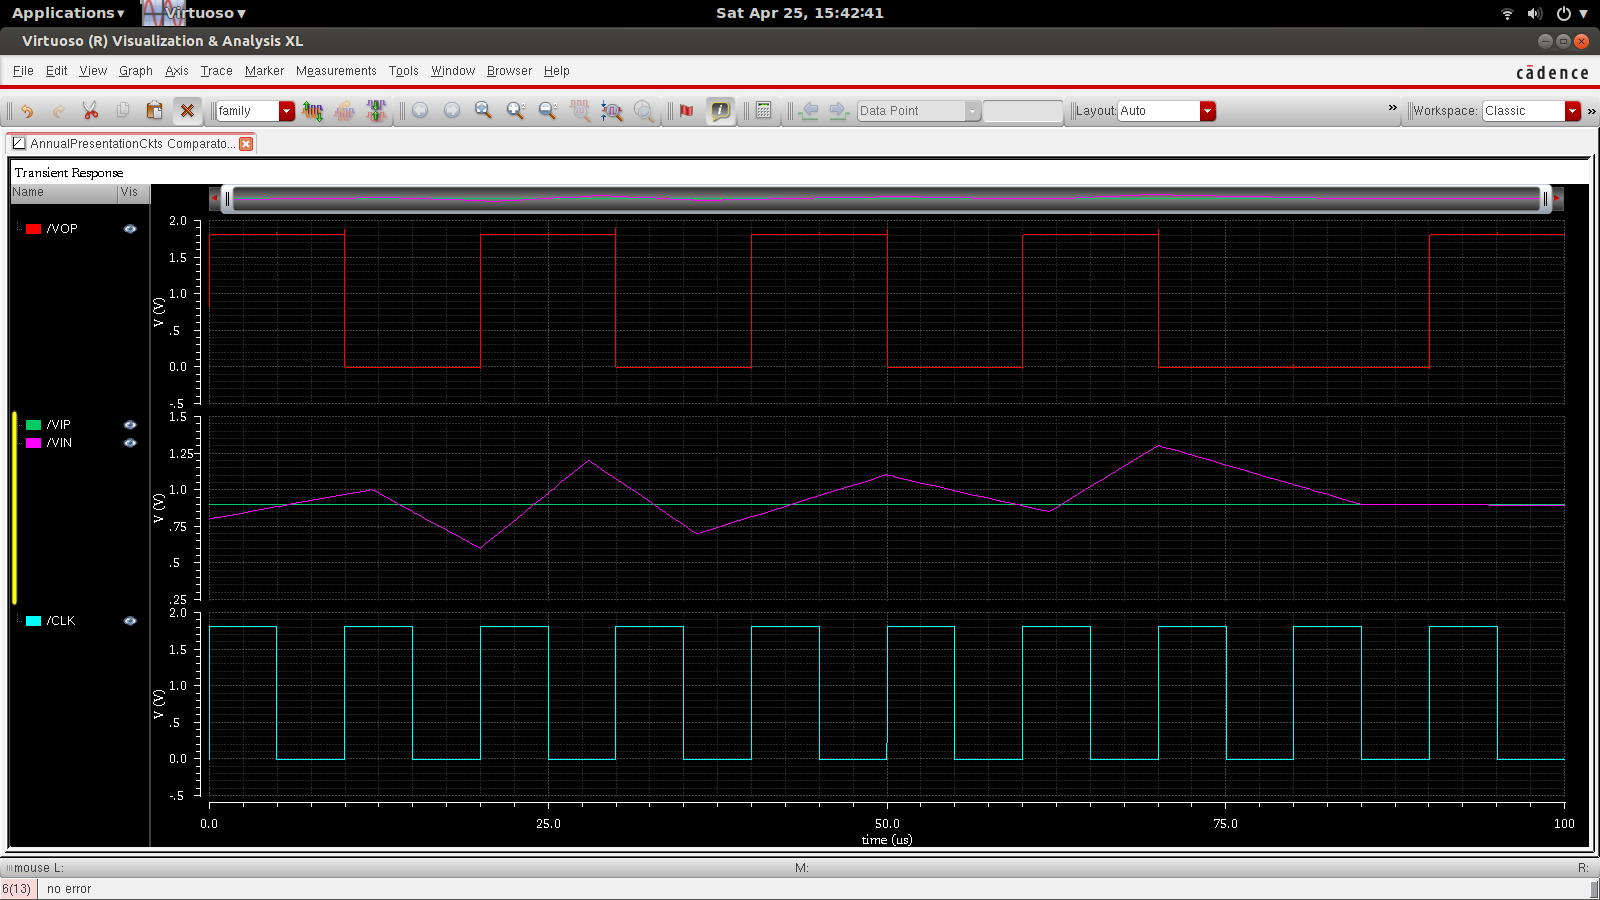
\includegraphics[width=10 cm]{Figures/SCMP.png}\\
		\end{figure}
		\scriptsize{ \color{blue}{}}
	\end{center}
\end{frame}
%---------------------------------------------------------------------------------------------------------------------------%
\begin{frame}
	\frametitle{Simulation results} \footnotesize
	\begin{center}
		\begin{figure}
			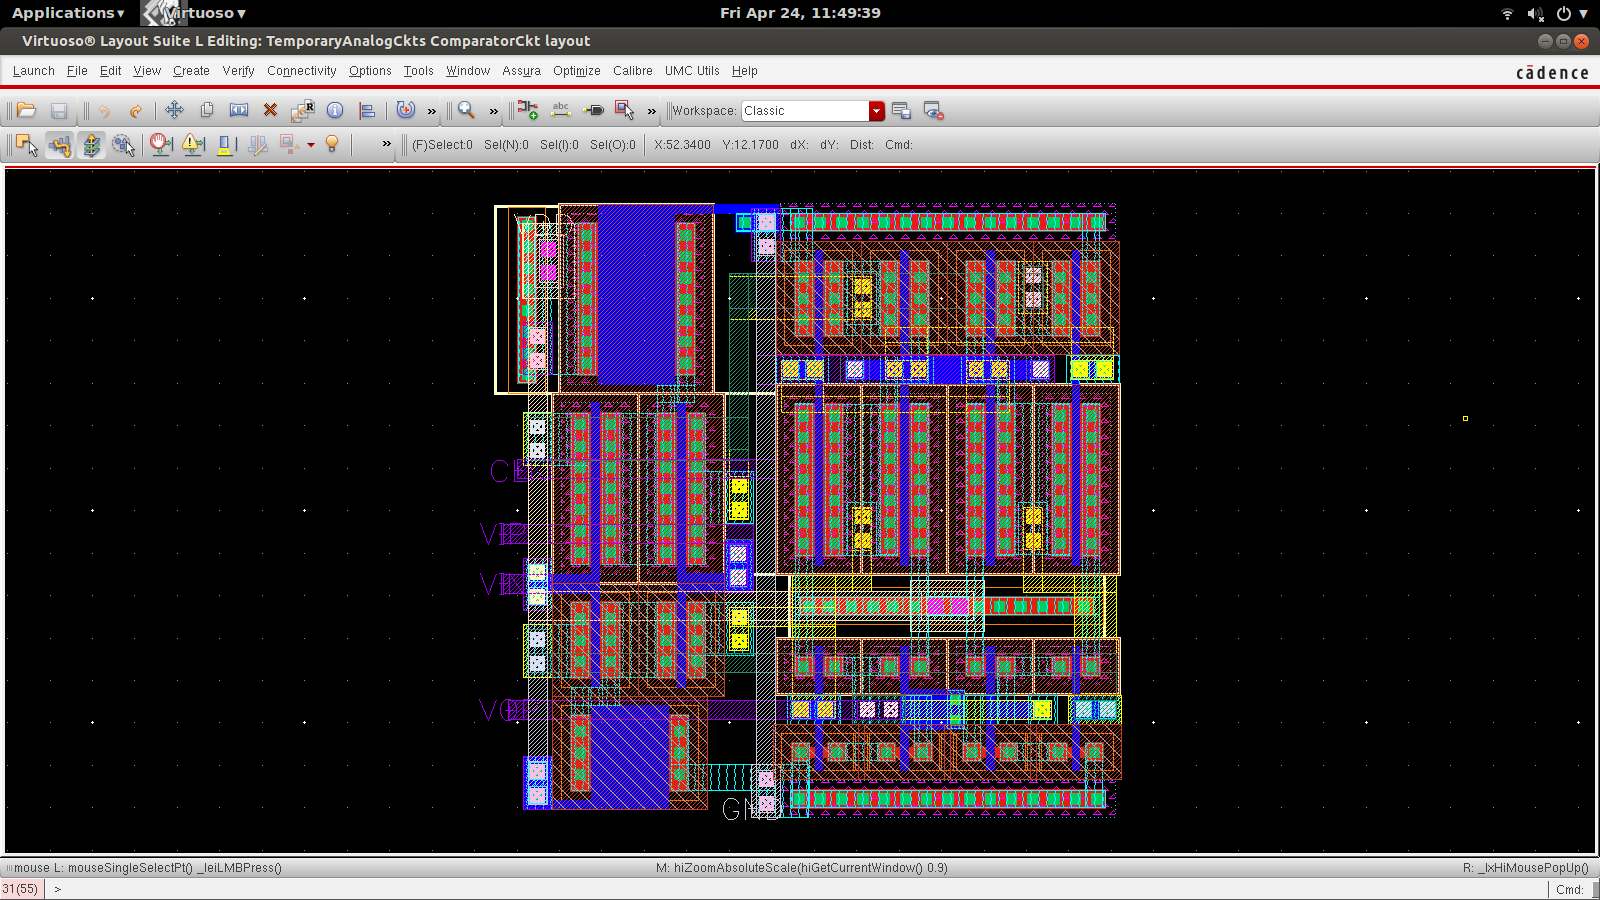
\includegraphics[width=10 cm]{Figures/LCMP.png}\\
		\end{figure}
		\scriptsize{ \color{blue}{}}
	\end{center}
\end{frame}
%---------------------------------------------------------------------------------------------------------------------------%
\begin{frame}
	\frametitle{Simulation results} \footnotesize
	\begin{center}
		\begin{figure}
			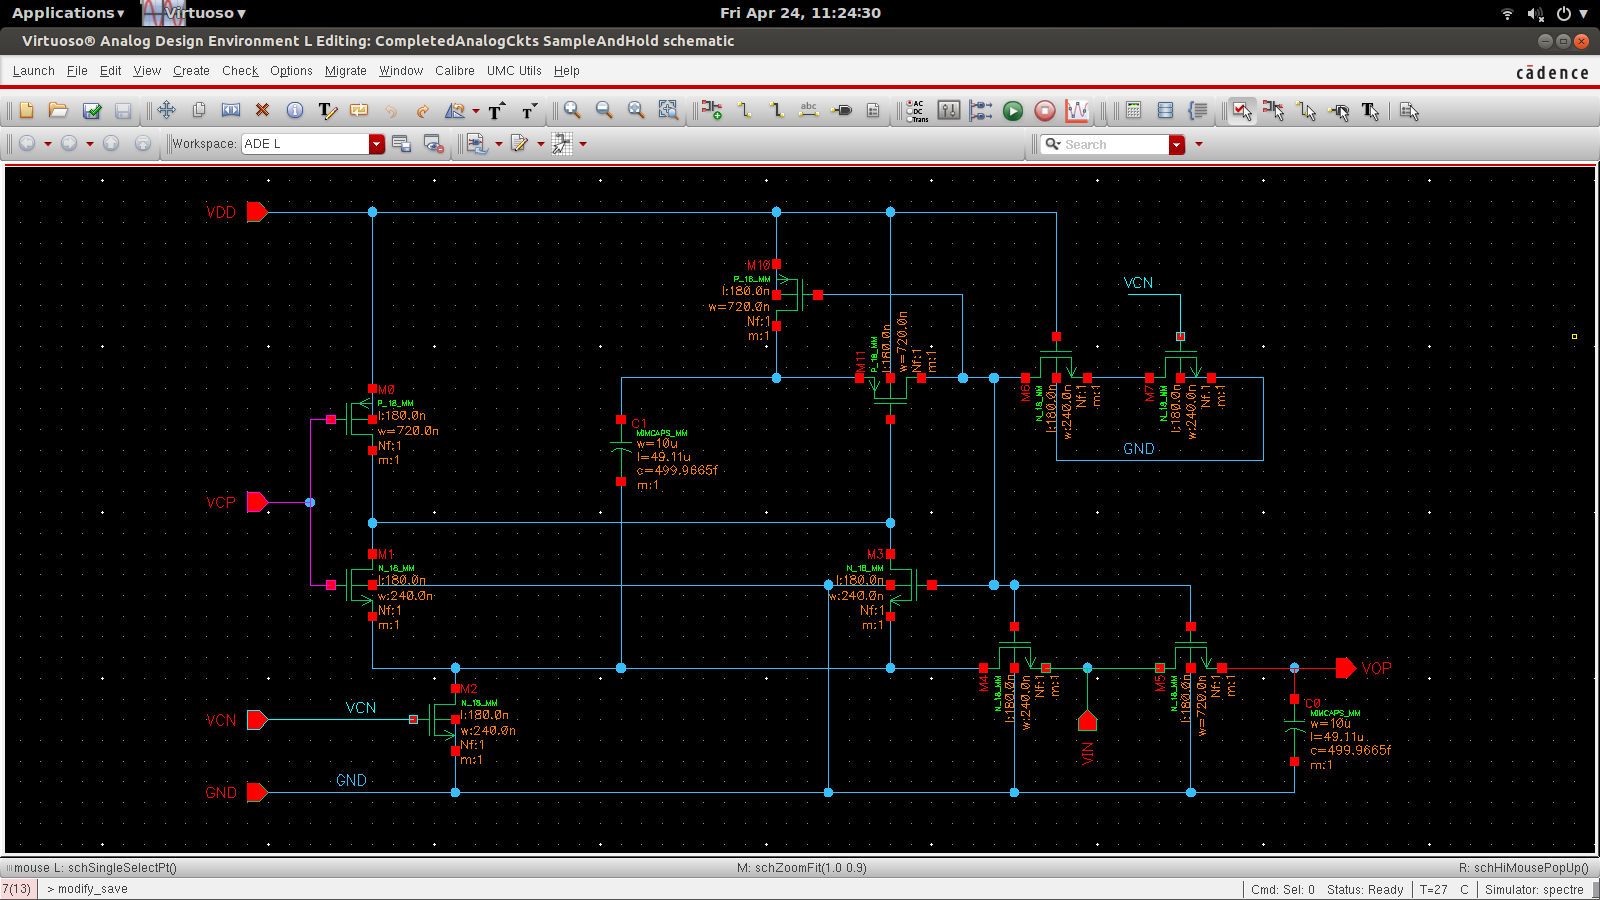
\includegraphics[width=10 cm]{Figures/CSAH.png}\\
		\end{figure}
		\scriptsize{ \color{blue}{}}
	\end{center}
\end{frame}
%---------------------------------------------------------------------------------------------------------------------------%
\begin{frame}
	\frametitle{Simulation results} \footnotesize
	\begin{center}
		\begin{figure}
			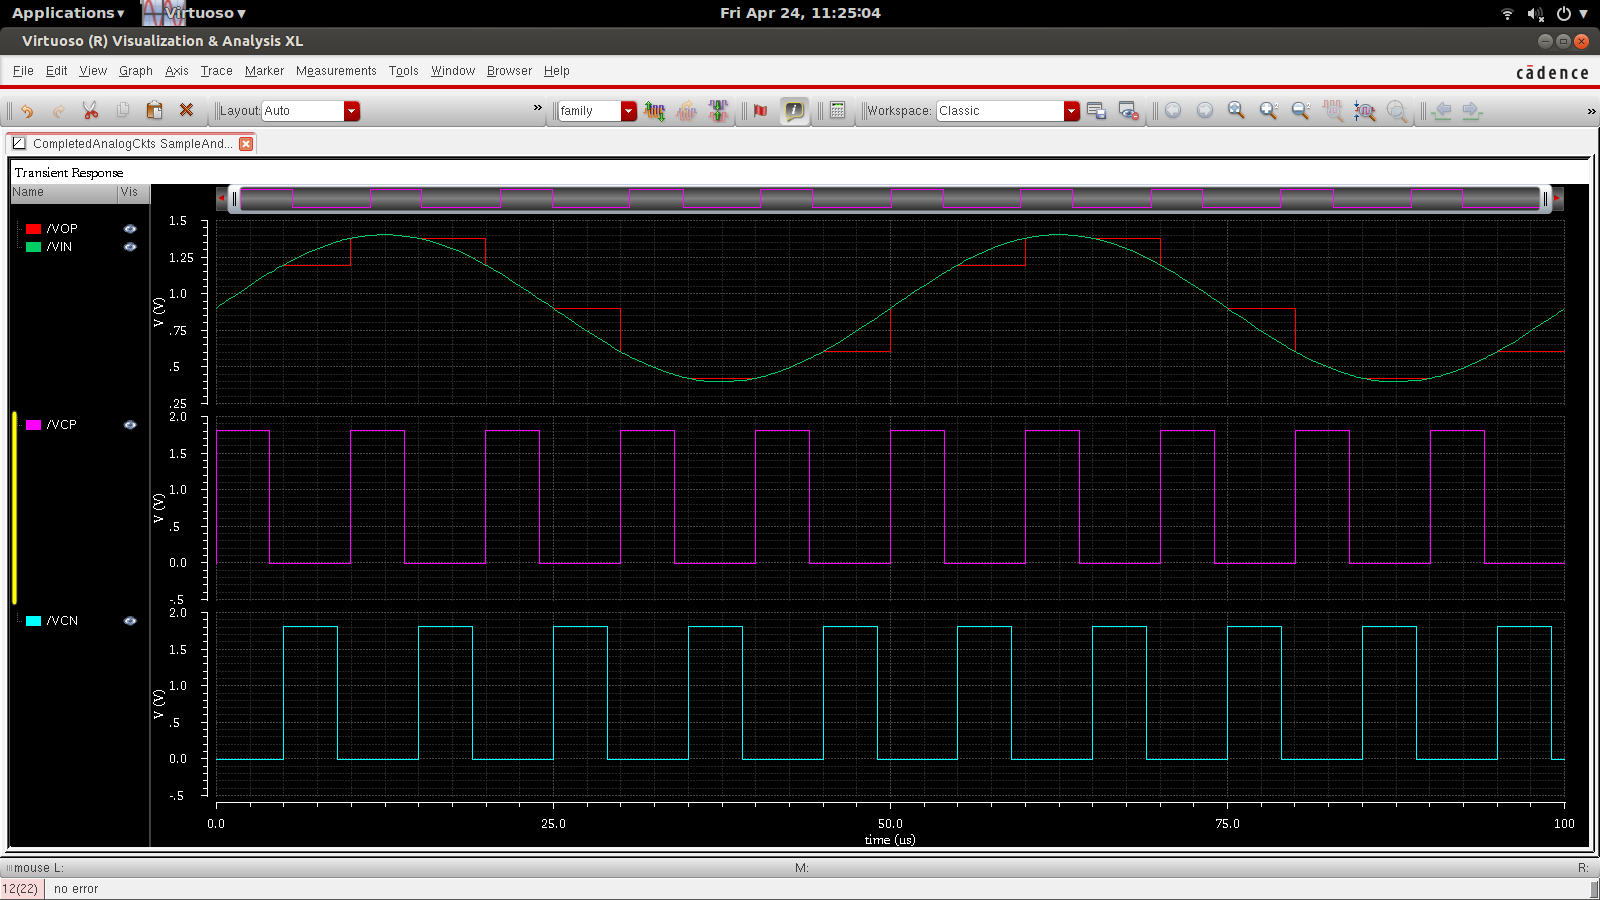
\includegraphics[width=10 cm]{Figures/SSAH.png}\\
		\end{figure}
		\scriptsize{ \color{blue}{}}
	\end{center}
\end{frame}
%---------------------------------------------------------------------------------------------------------------------------%
\begin{frame}
	\frametitle{Simulation results} \footnotesize
	\begin{center}
		\begin{figure}
			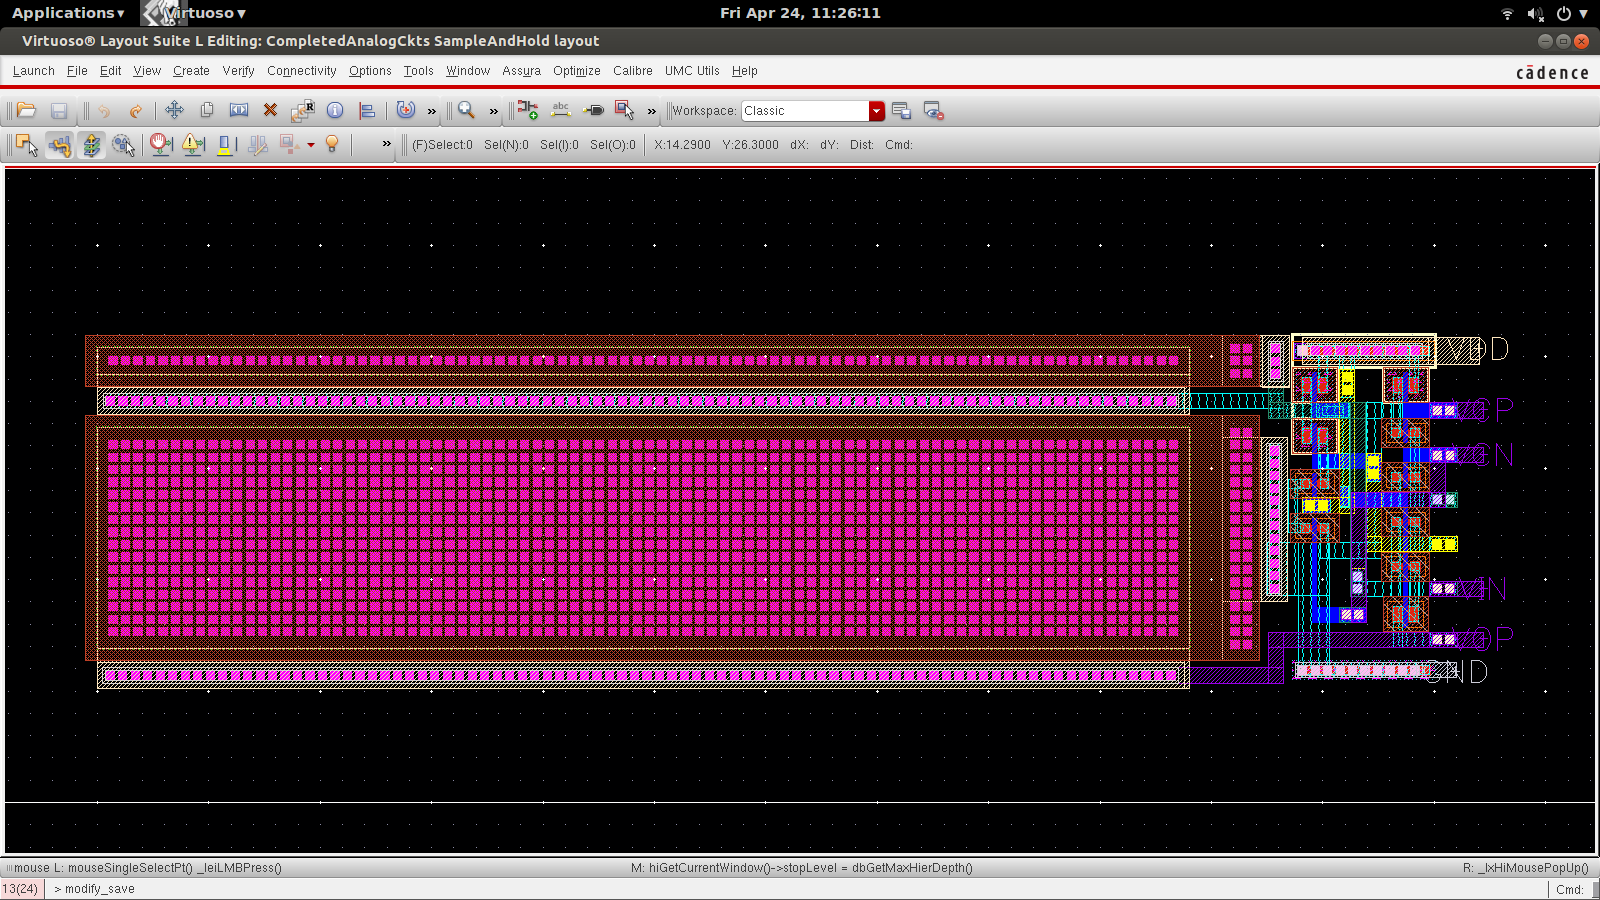
\includegraphics[width=10 cm]{Figures/LSAH.png}\\
		\end{figure}
		\scriptsize{ \color{blue}{}}
	\end{center}
\end{frame}
%---------------------------------------------------------------------------------------------------------------------------%
\begin{frame}
	\frametitle{Simulation results} \footnotesize
	\begin{center}
		\begin{figure}
			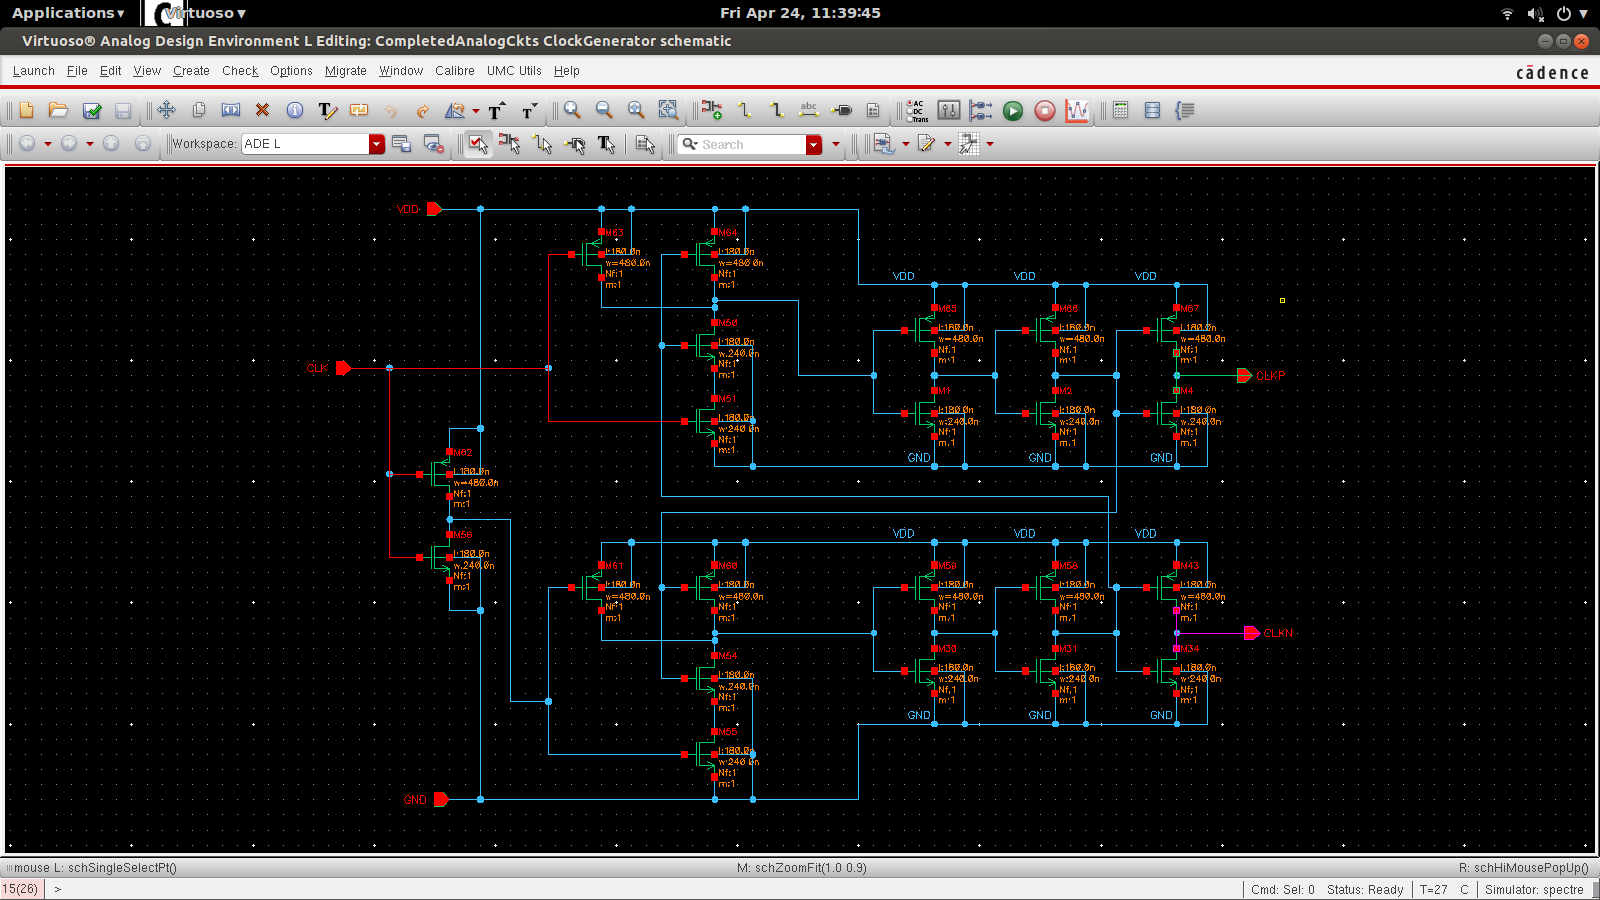
\includegraphics[width=10 cm]{Figures/CNOC.png}\\
		\end{figure}
		\scriptsize{ \color{blue}{}}
	\end{center}
\end{frame}
%---------------------------------------------------------------------------------------------------------------------------%
\begin{frame}
	\frametitle{Simulation results} \footnotesize
	\begin{center}
		\begin{figure}
			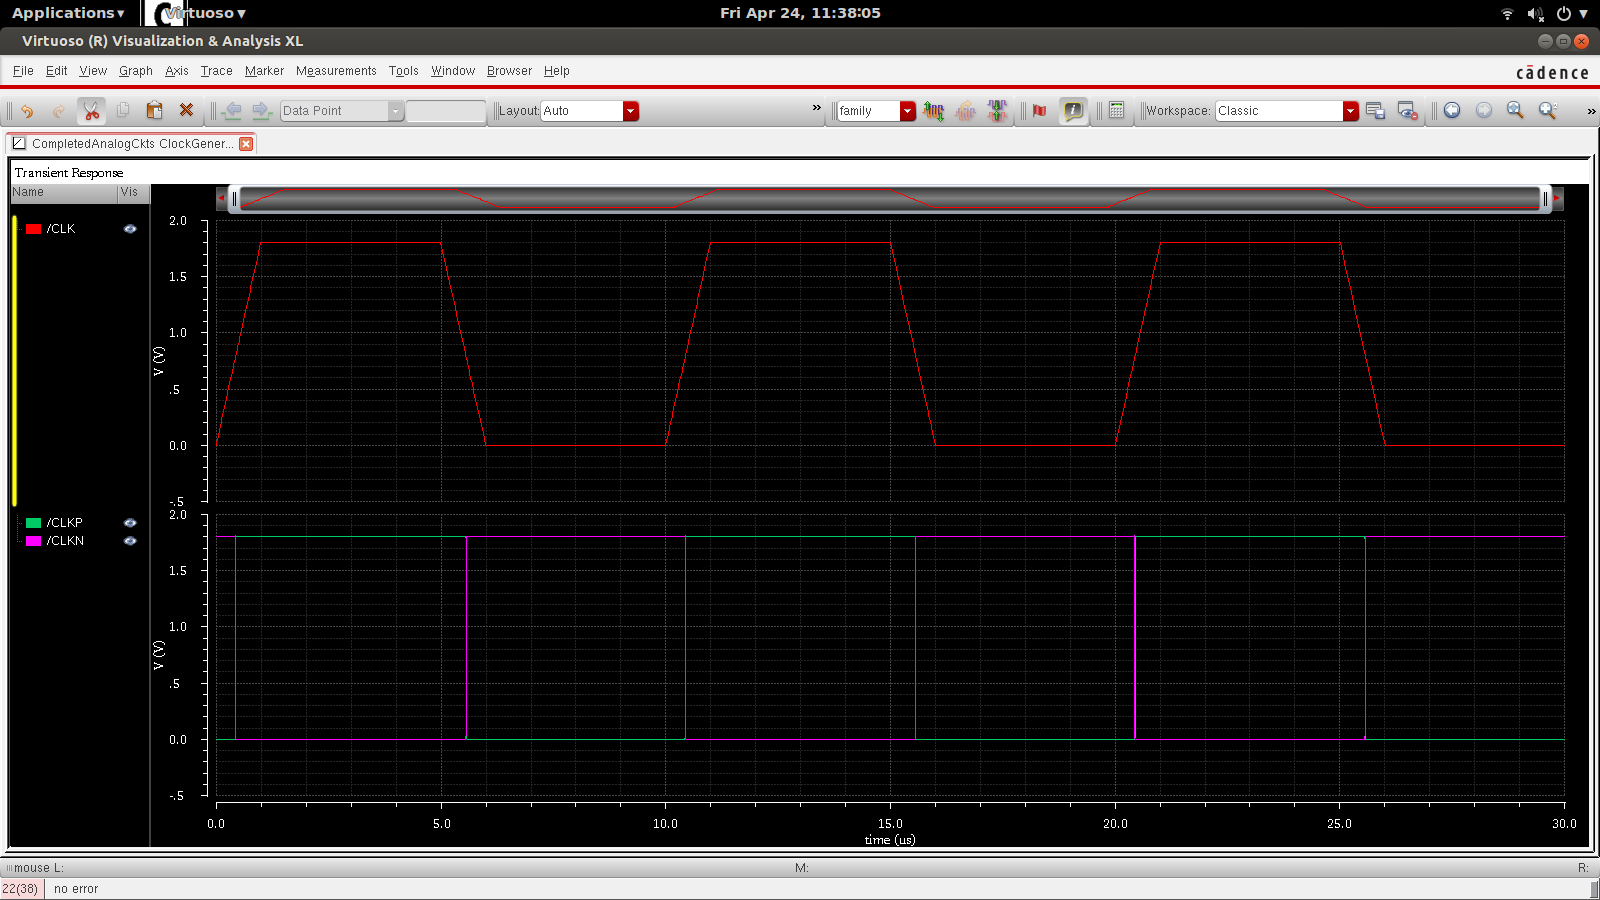
\includegraphics[width=10 cm]{Figures/SNOC.png}\\
		\end{figure}
		\scriptsize{ \color{blue}{}}
	\end{center}
\end{frame}
%---------------------------------------------------------------------------------------------------------------------------%
\begin{frame}
	\frametitle{Simulation results} \footnotesize
	\begin{center}
		\begin{figure}
			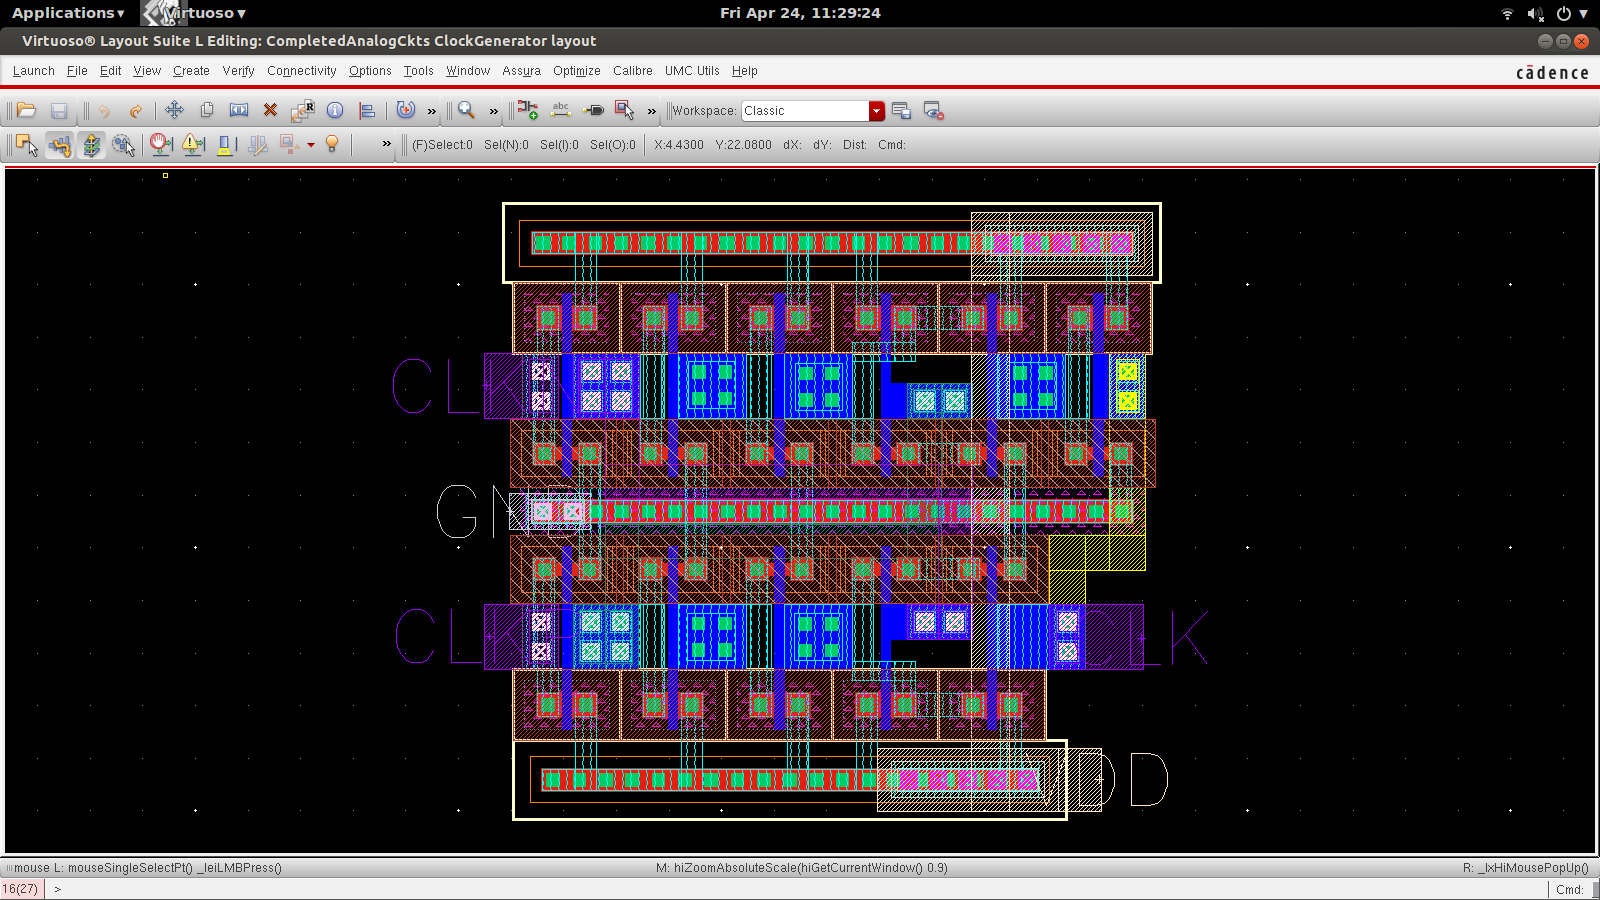
\includegraphics[width=10 cm]{Figures/LNOC.png}\\
		\end{figure}
		\scriptsize{ \color{blue}{}}
	\end{center}
\end{frame}
%---------------------------------------------------------------------------------------------------------------------------% %%%
\begin{frame}
	\frametitle{Simulation results} \footnotesize
	\begin{center}
		\begin{figure}
			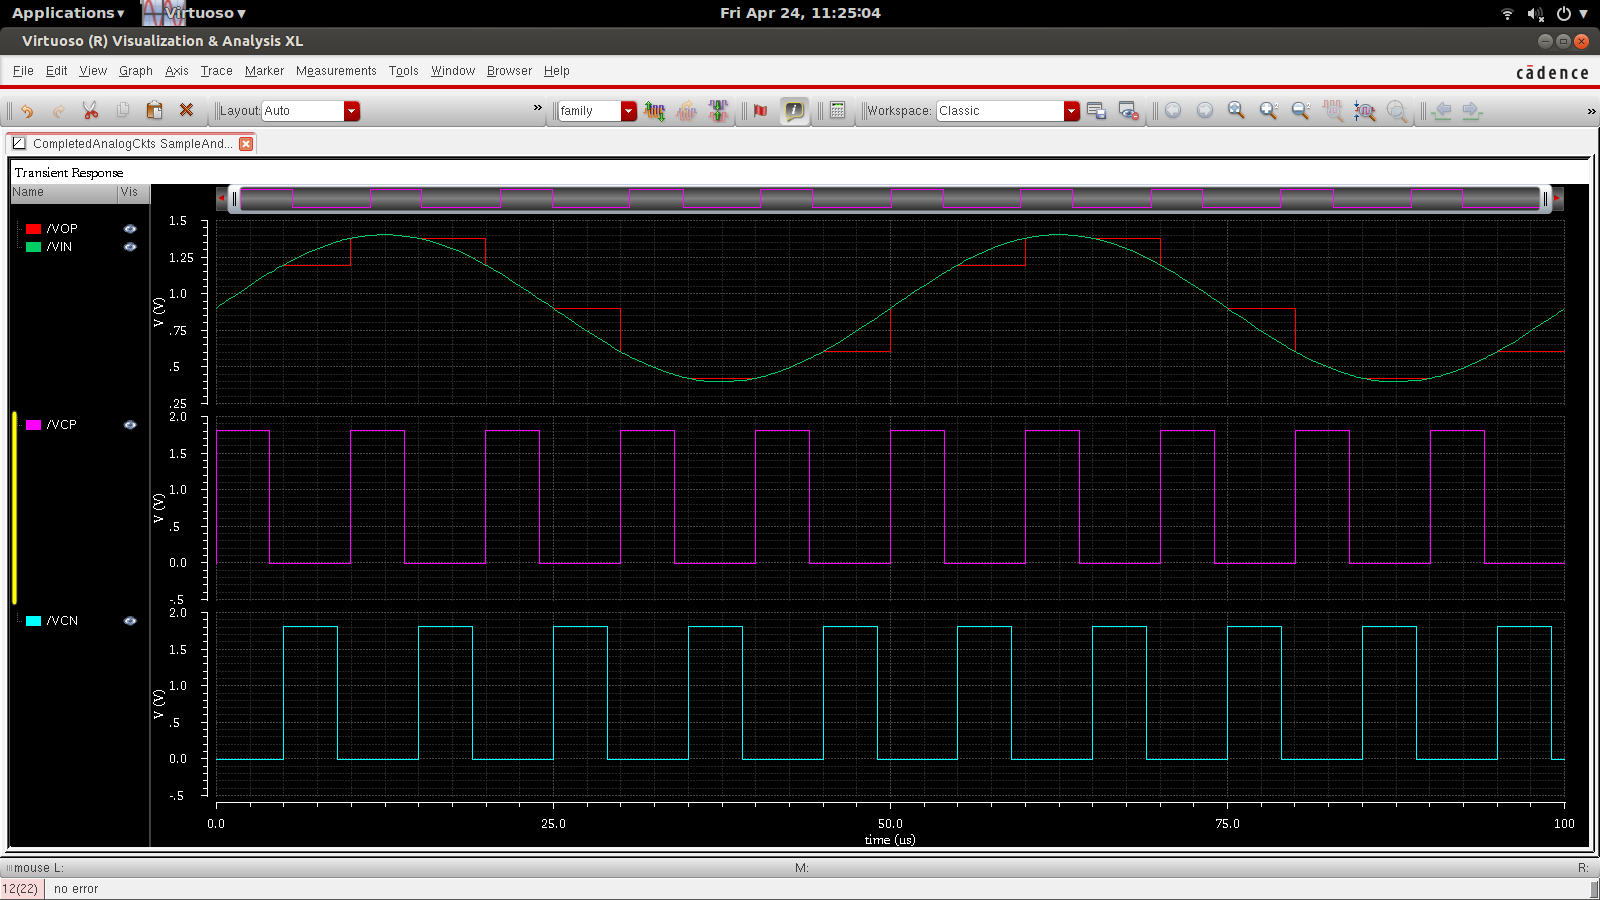
\includegraphics[width=10 cm]{Figures/SSAH.png}\\
		\end{figure}
		\scriptsize{ \color{blue}{}}
	\end{center}
\end{frame}
%---------------------------------------------------------------------------------------------------------------------------%
\begin{frame}
	\frametitle{Simulation results} \footnotesize
	\begin{center}
		\begin{figure}
			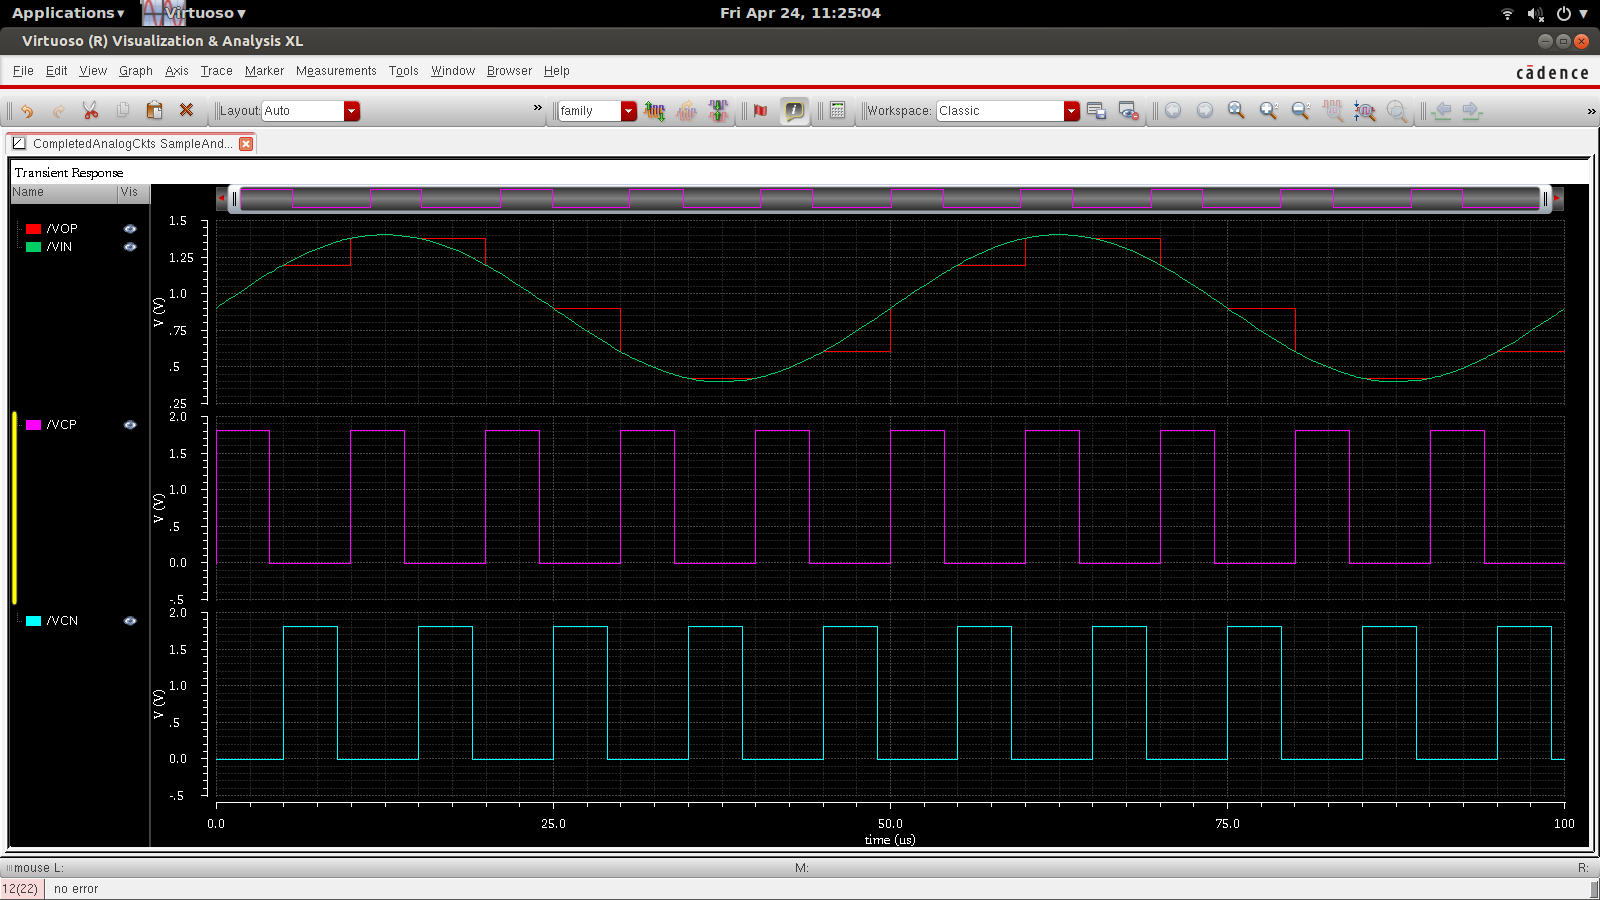
\includegraphics[width=10 cm]{Figures/SSAH.png}\\
		\end{figure}
		\scriptsize{ \color{blue}{}}
	\end{center}
\end{frame}
%---------------------------------------------------------------------------------------------------------------------------%
\begin{frame}
	\frametitle{Simulation results} \footnotesize
	\begin{center}
		\begin{figure}
			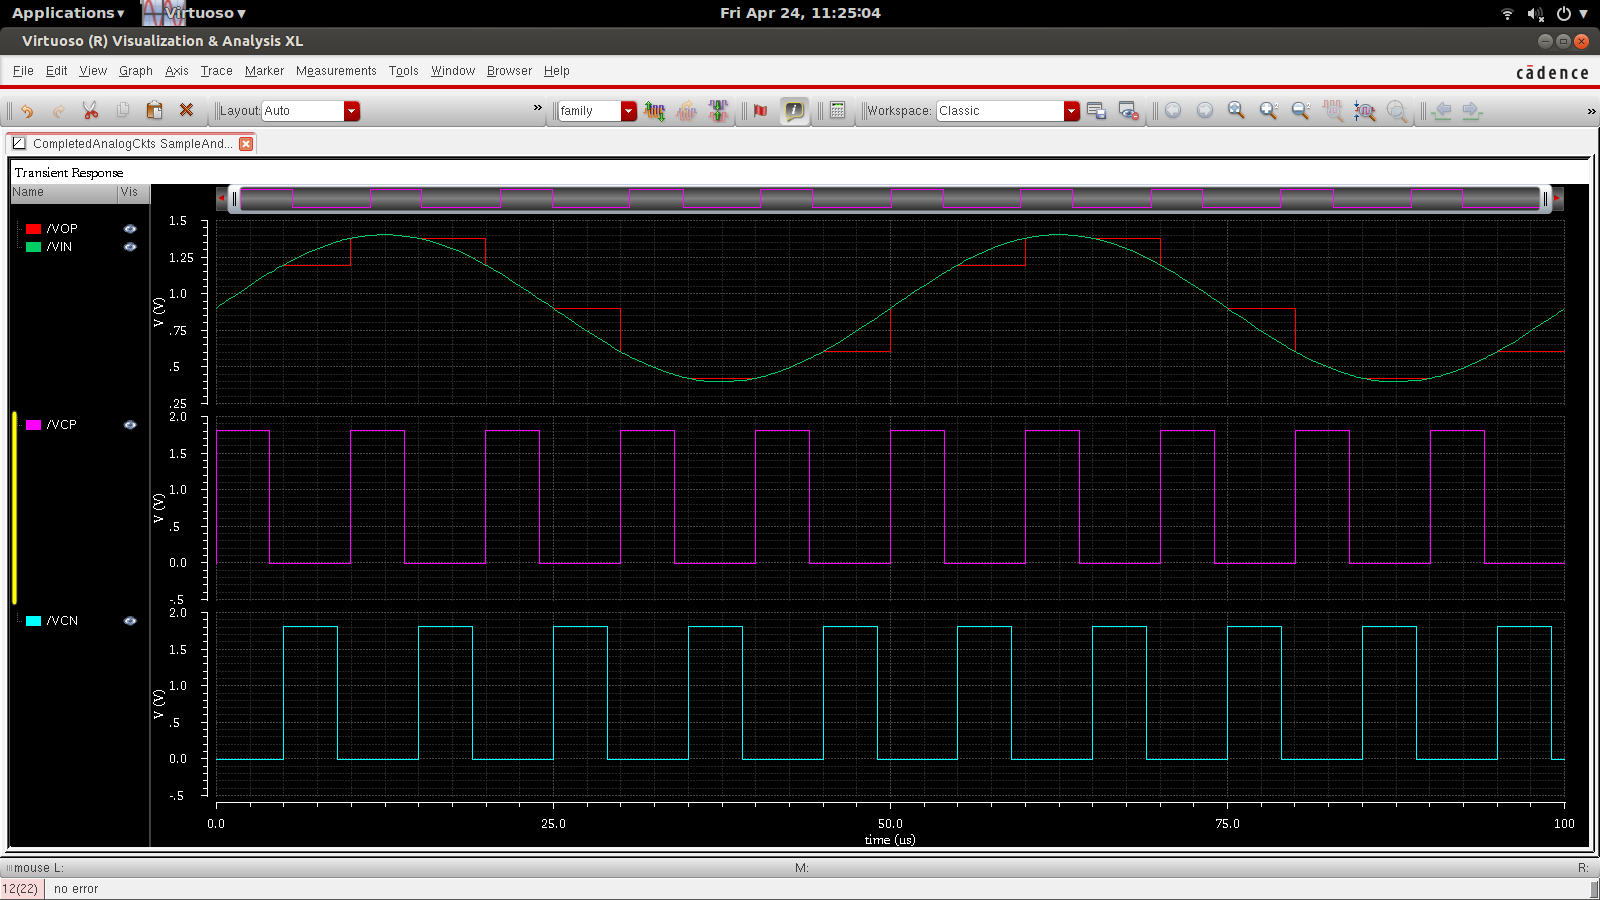
\includegraphics[width=10 cm]{Figures/SSAH.png}\\
		\end{figure}
		\scriptsize{ \color{blue}{}}
	\end{center}
\end{frame}
%---------------------------------------------------------------------------------------------------------------------------%







\begin{frame}
	\frametitle{Circuit diagram of proposed ADC architecture} \footnotesize
	\begin{center}
		\begin{figure}
			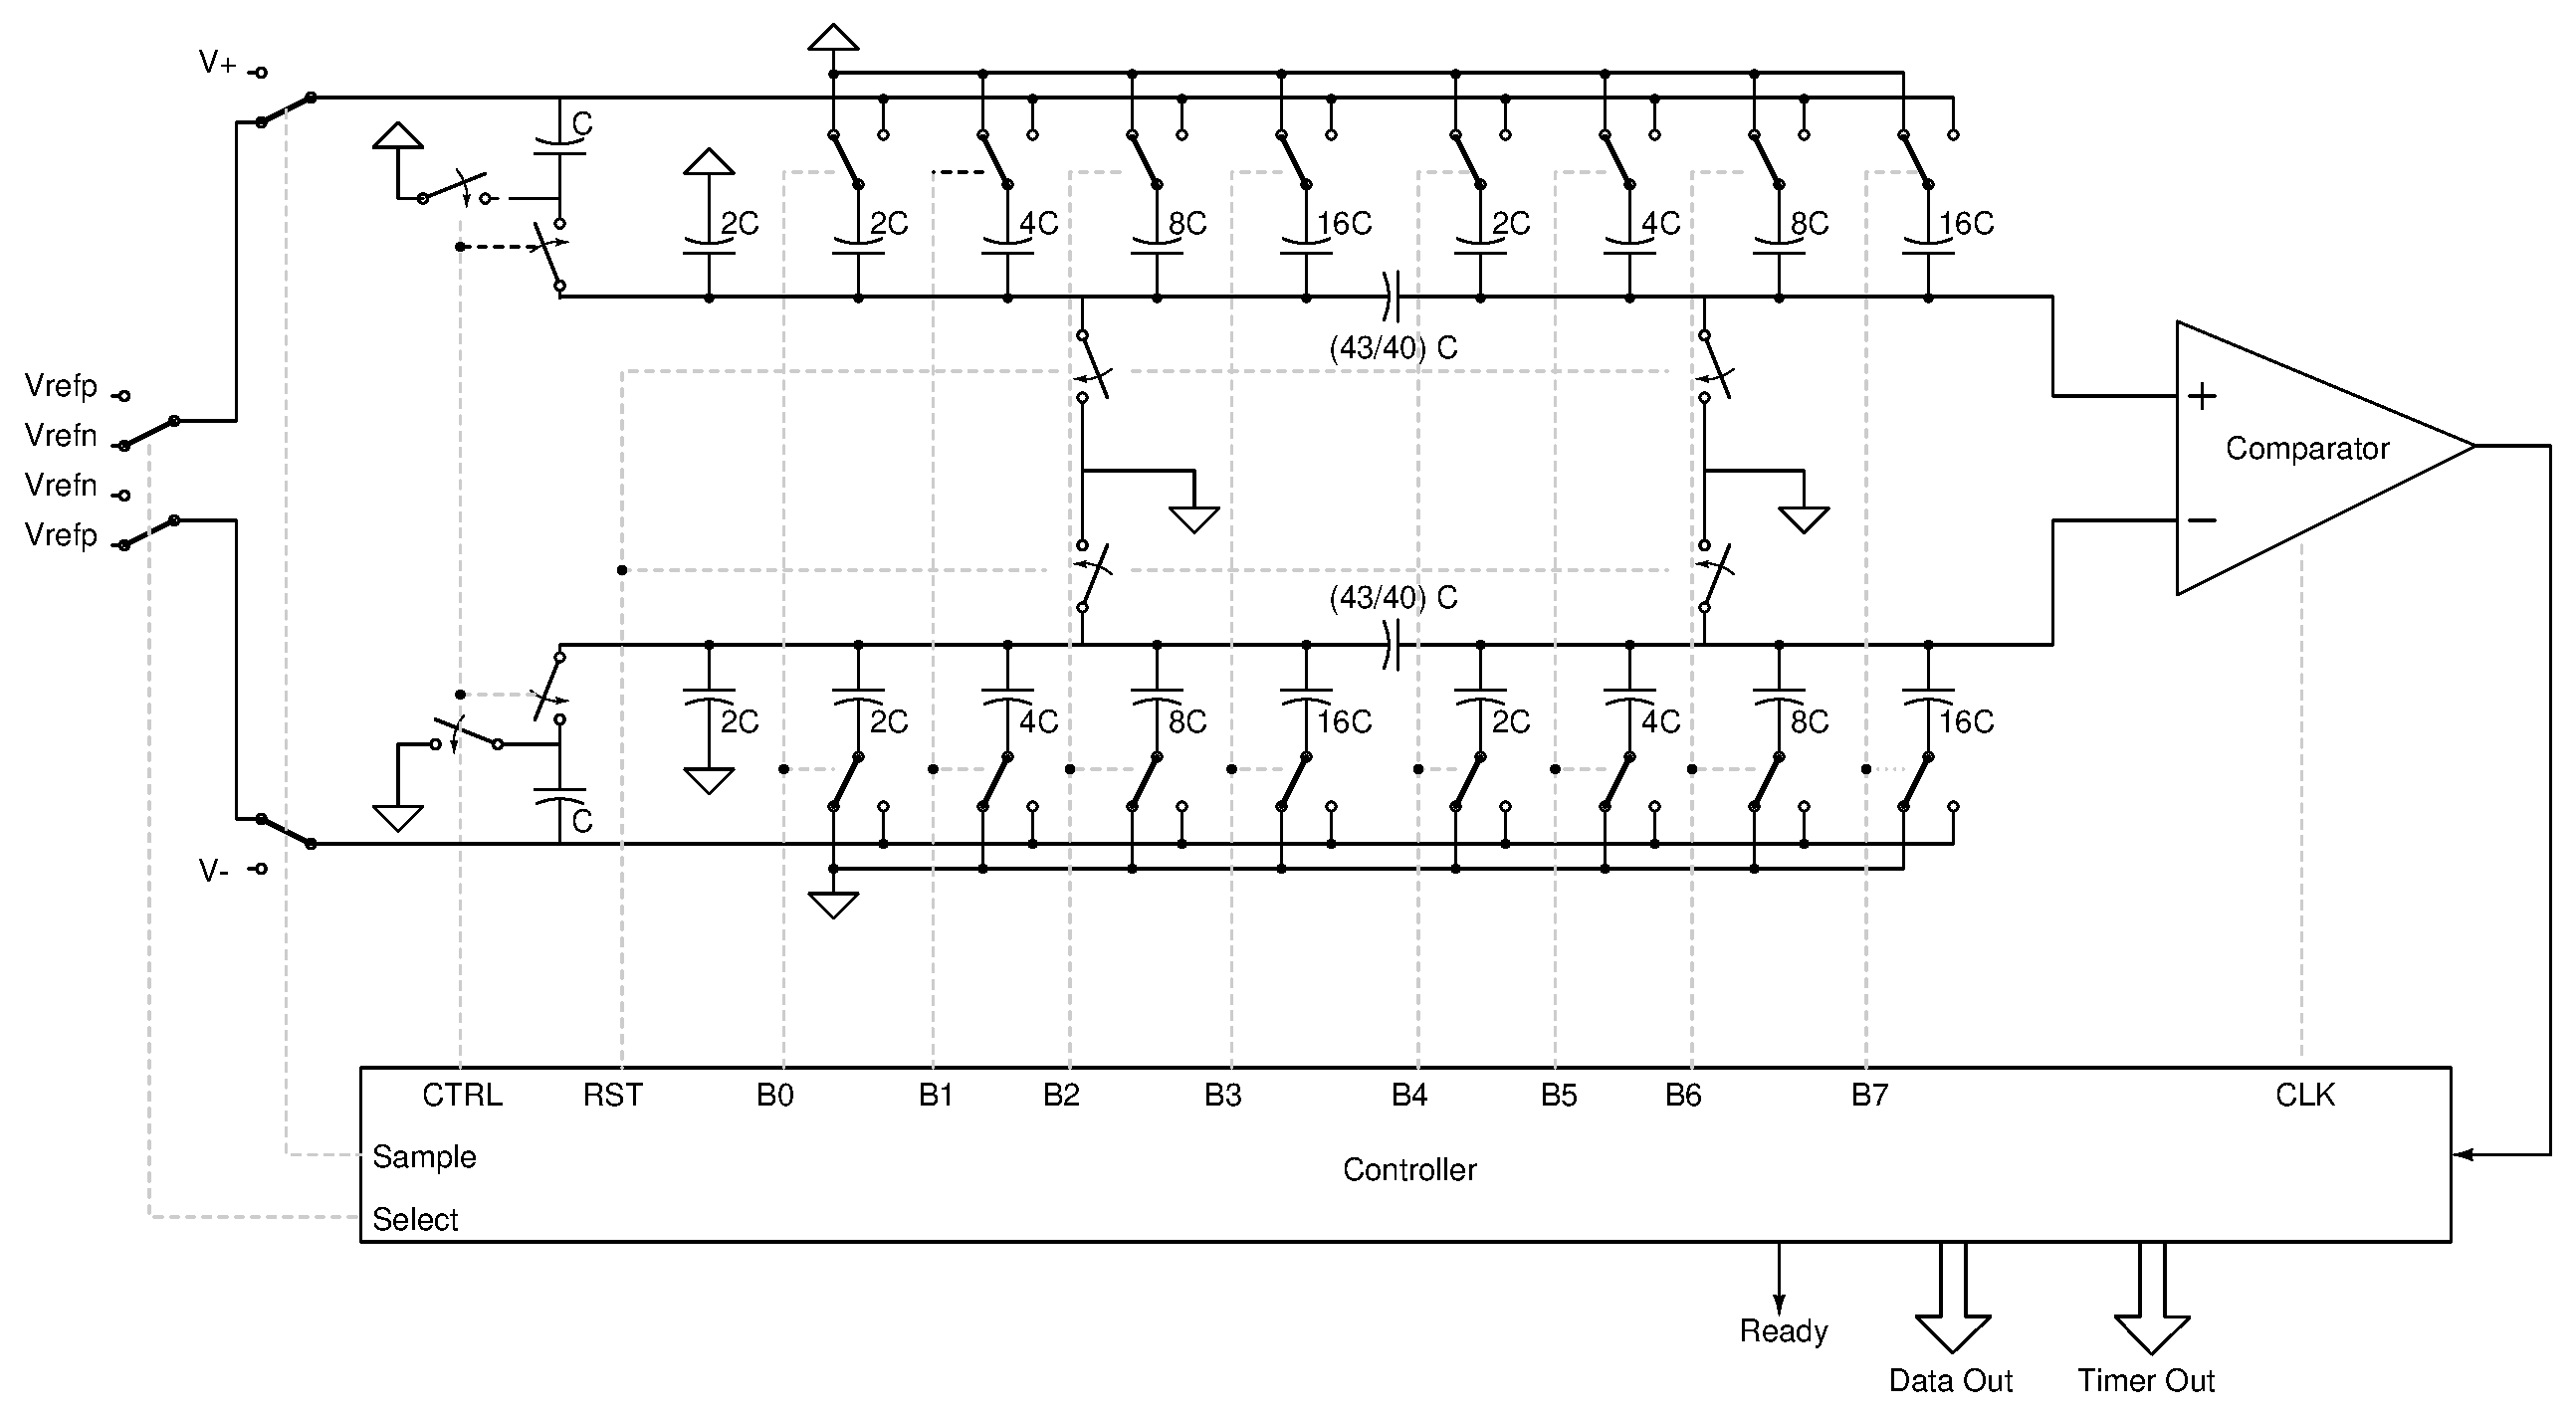
\includegraphics[width=10 cm,height=6 cm,angle=360]{Figures/15ADCfull.ps}\\
		\end{figure}
		\scriptsize{ \color{blue}{Proposed level crossing ADC circuit diagram}}
	\end{center}
\end{frame}
%---------------------------------------------------------------------------------------------------------------------------%
\begin{frame}
	\frametitle{Building blocks for proposed level crossing ADC} \footnotesize
	\begin{itemize} 
		\item{ ADC specifications}
			\begin{itemize} \scriptsize
				\item{ Technology - UMC 180nm } \\
				\item{ Power supply - 1.8 V } \\
				\item{ Resolution - 8-bit  } \\
				\item{ Peak to peak analog input voltage - 1 V (0.4 to 1.4)} \\
				\item{ Maximum analog input frequency - 20K Hz } \\
			\end{itemize}
		\item{ Analog Blocks }\\
			\begin{itemize} \scriptsize
				\item{ Clocked Comparator } \\
				\item{ Track \& Hold } \\
				\item{ Non overlapping clock generator } \\
				\item{ Switching network for capacitor array } \\
				\item{ Capacitor array  } \\
			\end{itemize}
		\item{ Digital Blocks }
			\begin{itemize} \scriptsize
				\item{ Controller for high activity signals } \\
				\item{ Controller for low activity signals } \\
			\end{itemize}	
	\end{itemize}
\end{frame}
%---------------------------------------------------------------------------------------------------------------------------%
\begin{frame}
	\frametitle{Building blocks for proposed level crossing ADC} \footnotesize
	\begin{itemize}  
		\item{ Capacitor array is implemented using MIM capacitors. } \\
		\item{ Switches for Capacitor array are implemented using analog MUX. } \\
		\item{ Split capacitor array method is used in Capacitor array for DAC. } \\
		\item{ Digital blocks are implemented using Faraday design kit. } \\
		\item{ Present status in implementation. } \\
			\begin{itemize} \scriptsize
				\item{ Clocked Comparator - Layout Completed} \\
				\item{ Track \& Hold - Layout Completed} \\
				\item{ Non overlapping clock generator - Layout Completed} \\
				\item{ Switching network for capacitor array - Layout in process} \\
				\item{ Capacitor array - Layout in process } \\
			\end{itemize}
	\end{itemize}
\end{frame}
%---------------------------------------------------------------------------------------------------------------------------%
\begin{frame}
	\frametitle{Building blocks for proposed level crossing ADC} \footnotesize
	\begin{center}
		\begin{figure}
			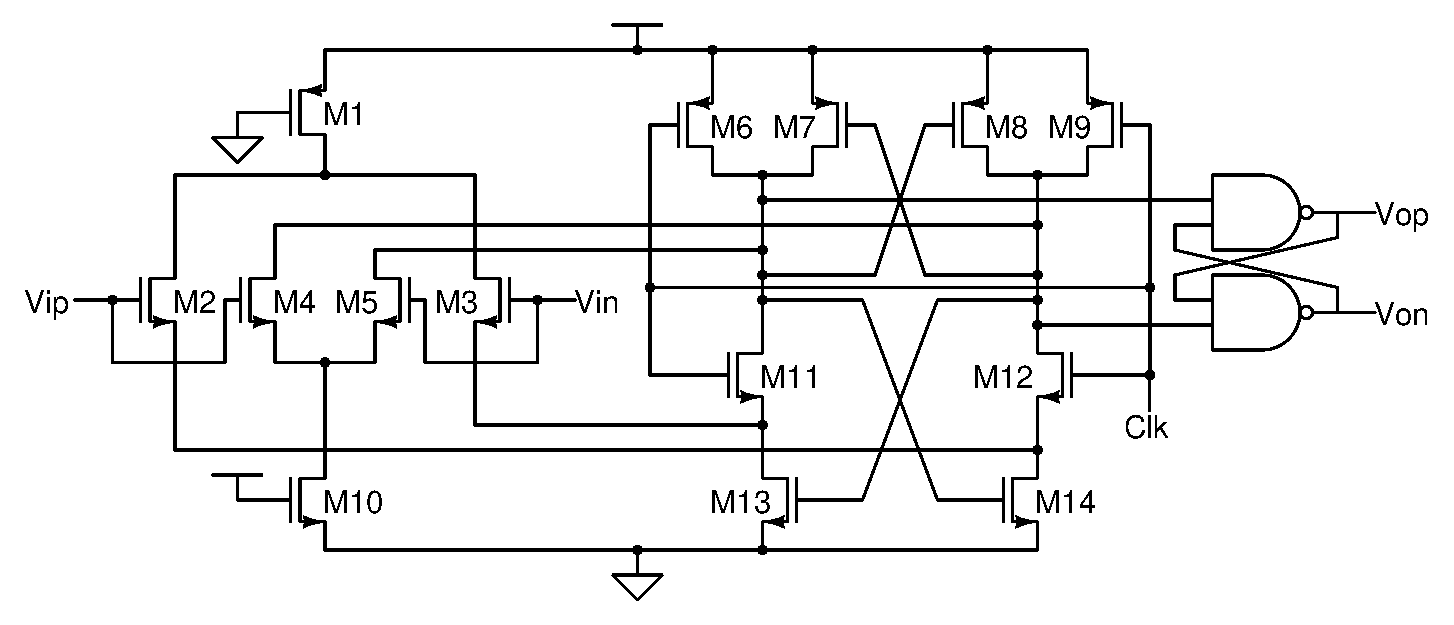
\includegraphics[width=10 cm]{Figures/CMP.eps}\\
		\end{figure}
		\scriptsize{ \color{blue}{Clocked Comparator used in proposed ADC architecture}}
	\end{center}
\end{frame}
%---------------------------------------------------------------------------------------------------------------------------%
\begin{frame}
	\frametitle{Building blocks for proposed level crossing ADC} \footnotesize
	\begin{center}
		\begin{figure}
			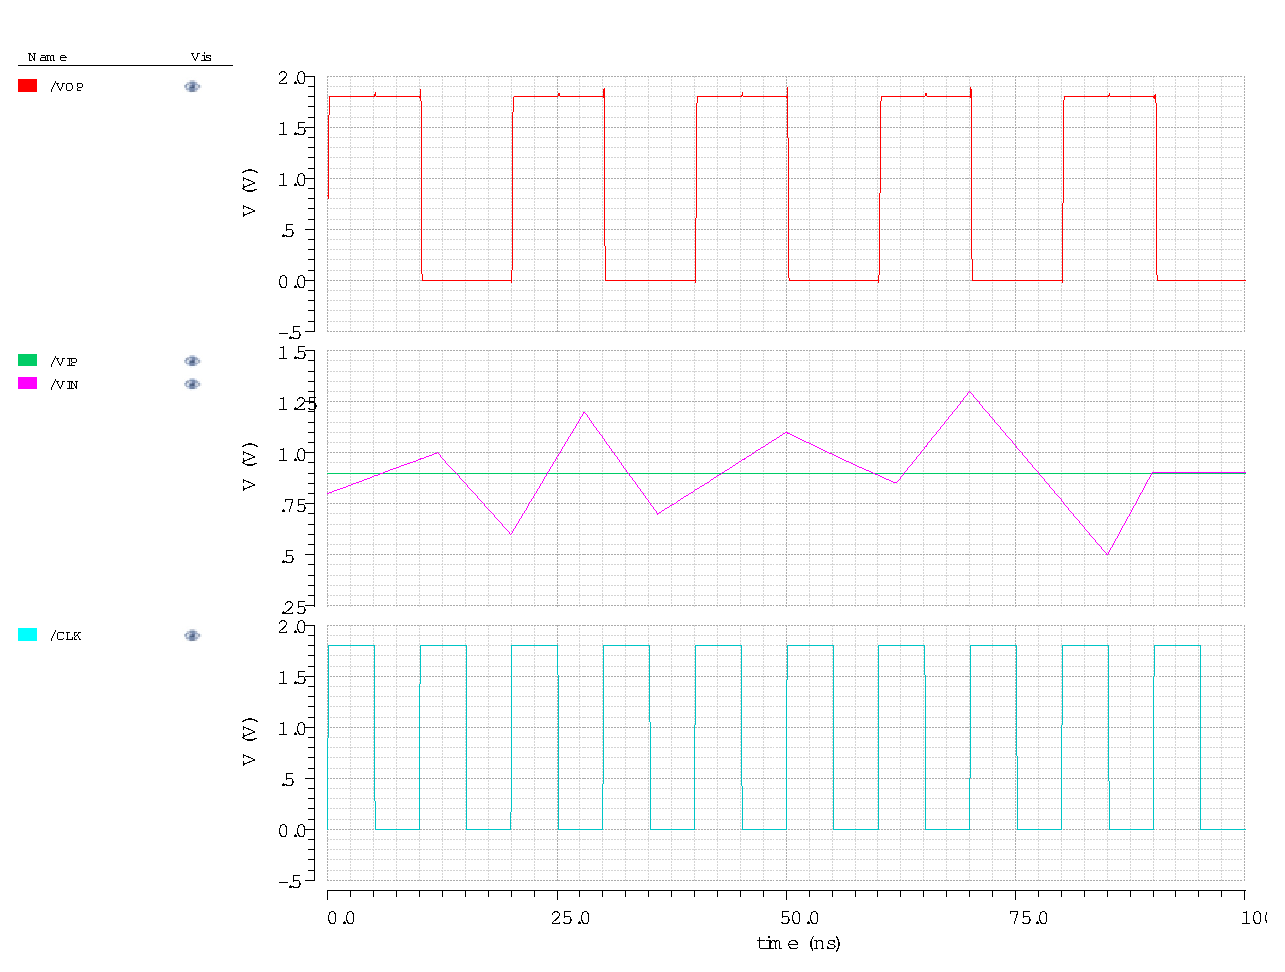
\includegraphics[width=10 cm, height=6 cm, angle=360]{Figures/SCMP.eps}\\
		\end{figure}
		\scriptsize{ \color{blue}{Simulation results of Clocked Comparator used in proposed ADC architecture}}
	\end{center}
\end{frame}
%---------------------------------------------------------------------------------------------------------------------------%
\begin{frame}
	\frametitle{Building blocks for proposed level crossing ADC} \footnotesize
	\begin{center}
		\begin{figure}
			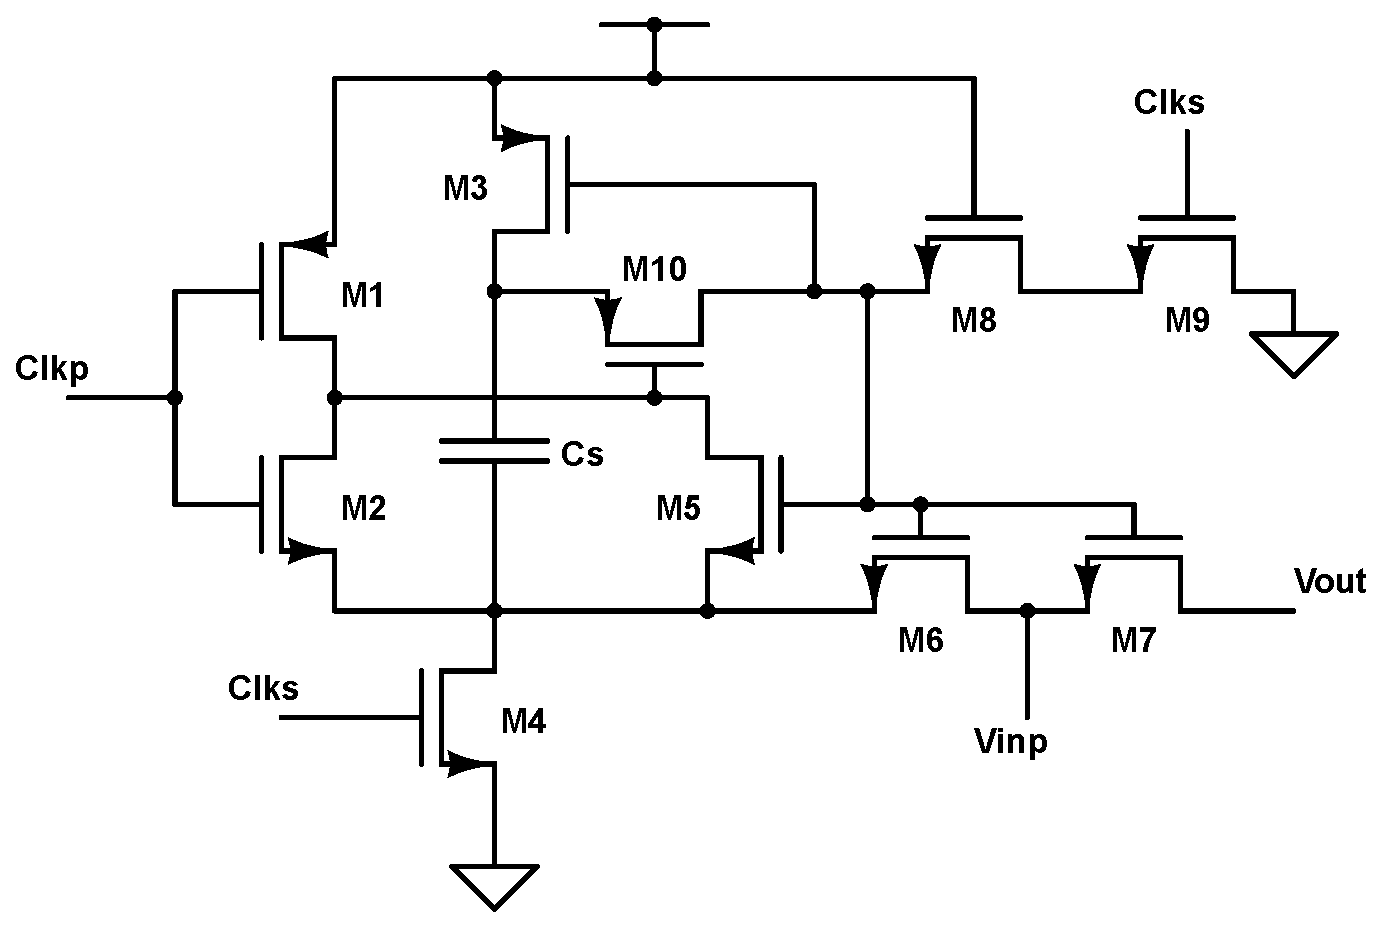
\includegraphics[width=7 cm]{Figures/TAH.eps} \\
		\end{figure}
		\scriptsize{ \color{blue}{Track and Hold used in proposed ADC architecture}}
	\end{center}
\end{frame}
%---------------------------------------------------------------------------------------------------------------------------%
\begin{frame}
	\frametitle{Building blocks for proposed level crossing ADC} \footnotesize
	\begin{center}
		\begin{figure}
			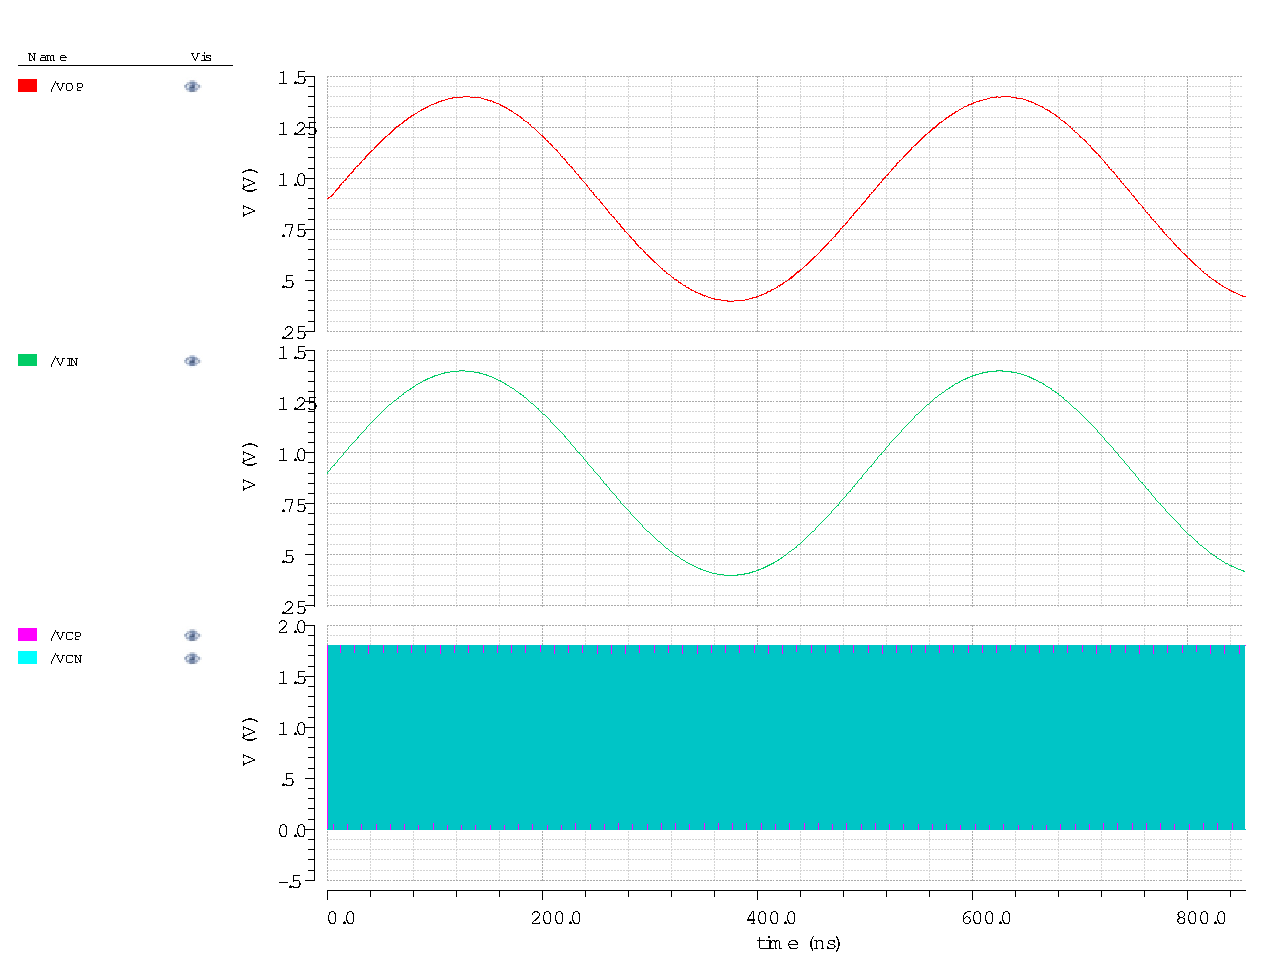
\includegraphics[width=10 cm, height=6 cm,angle=360]{Figures/STAH.eps}\\
		\end{figure}
		\scriptsize{ \color{blue}{Simulation results of Track and Hold used in proposed ADC architecture}}
	\end{center}
\end{frame}
%---------------------------------------------------------------------------------------------------------------------------%
